
This chapter introduces fundamental concepts of machine learning and deep learning that underpin the waveform classification task addressed in this thesis. It begins with linear regression, a foundational method familiar to most physicists, to illustrate basic supervised learning principles.
Next, the multilayer perceptron (MLP) is presented as a foundational neural network model to introduce core deep learning principles, such as optimization techniques and the backpropagation algorithm. 
Finally, the chapter explores the Transformer architecture, focusing on the encoder component, which is most relevant for waveform classification tasks like those in LEGEND-200. Core components of Transformer networks, such as positional encoding and the attention mechanism are explained, as they are essential for modeling the temporal structure of waveform data. 

\subsection{Machine learning and deep learning}
There is no fixed definition of Artificial Intelligence (AI), but it usually describes systems that simulate intelligent behavior. Machine learning (ML) is a subfield of AI concerned with constructing mathematical models that learn patterns from data to perform tasks such as classifying events or estimating continuous quantities~\cite{badillo_introduction_2020, prince_understanding_2023}. 
ML algorithms are commonly grouped into several paradigms. Two of the most widely used are:

a) Unsupervised learning: Only the input data is available, and the goal is to discover structure without labeling targets. Typical techniques are clustering (partitioning data into similar subsets) and dimensionality reduction (compressing data while preserving salient information)~\cite{badillo_introduction_2020}. 

b) Supervised learning: Models learn a mapping $f(x, \boldsymbol{\theta})$ from inputs $x$ to known targets $y$. If $y$ takes discrete values (e.g., classifying a waveform as signal or background), the problem is one of classification; if $y$ is continuous, it is a regression task~\cite{prince_understanding_2023, badillo_introduction_2020}. 


To illustrate these concepts concretely, consider a one-dimensional linear regression, where the goal is to find a mapping of the form:

\begin{equation}
\label{eq:linear_regression}
	f(x, \boldsymbol{\theta}) =  \theta_0 + \theta_1 \cdot x \,.
\end{equation}

In general, $\theta_0$ is denoted as the bias, and $\theta_1$ is the weight. Simply, the goal is to find the parameter vector $\boldsymbol{\theta}$ that minimizes the discrepancy between the model predictions $f(x, \boldsymbol{\theta})$ and the true outputs $y_i$. A common choice is the sum of squared errors, known as least squares loss:

\begin{equation}
\label{eq:least_squares}
	L[\theta] = \sum_i^N \left( f(x_i, \boldsymbol{\theta}) - y_i \right)^2 \,.
\end{equation}

\noindent Minimizing this loss yields the optimal parameters $\hat{\boldsymbol{\theta}}$ for which the model's predictions best approximate the training data: 

\begin{equation}
\label{eq:optimize_loss_function} 
	\hat{\boldsymbol{\theta}} = \underset{\boldsymbol{\theta}}{\mathrm{argmin}} \; L\left[\boldsymbol{\theta}\right] \,.
\end{equation}

This procedure is referred to as training the model. Once trained, the model can be used to make predictions on new, unseen input data. If the model is too simple to capture the true underlying structure of the data, it is said to be underfitted. Conversely, if the model is excessively complex and learns noise or random fluctuations in the data, it is overfitted and likely to generalize poorly to unseen inputs~\cite{prince_understanding_2023}. 

\subsubsection{Multilayer perceptrons}
\label{sec:03_mlp}

Finding suitable features for machine learning models is often a challenging and time-consuming task. In fact, until recently, progress in machine learning was largely constrained not by model complexity but by the need for effective, manually crafted feature transformations. 
Deep learning (DL) addresses this limitation by integrating the feature transformation step directly into the model itself~\cite{lecun_deep_2015}. Instead of requiring handcrafted input features, DL models learn them automatically from raw data. This is accomplished by introducing additional parameters $\boldsymbol{\vartheta}$ that govern the structure of the feature transform:  

\begin{equation}
\label{eq:dl_feature_transform}
	f(x; \boldsymbol{\theta}, \boldsymbol{\vartheta}) = \theta_0 + \theta_1 \cdot \phi(x; \boldsymbol{\vartheta})\,.
\end{equation}

The key idea is that a recursive composition of simple functions can model highly complex, non-linear mappings. Non-linearity in the functions is essential, as without it, the stacked layers would collapse to a single affine transformation. This is formalized by expressing the overall model as a composition of layers:

\begin{equation}
\label{eq:dl_recursive_feature_transform}
f(\mathbf{x}; \boldsymbol{\theta}) = f_L(f_{L-1}(\ldots f_1(\mathbf{x})) \ldots )) \,.
\end{equation}

where each $f_l$ represents a transformation at layer $l$, which often involves a linear mapping followed by a non-linear activation. The input vector $\mathbf{x}$ is successively transformed through these layers, enabling the network to extract hierarchical features of increasing complexity. Models that follow this idea are referred to as feedforward neural networks, or more specifically, multilayer perceptrons (MLPs)~\cite{lecun_deep_2015, murphy_probabilistic_2022}. 

At the core of these architectures lies the perceptron, a computational unit that performs a weighted sum of its inputs followed by a nonlinear activation. By arranging many such units in layers, MLPs are able to model a wide range of nonlinear functions through learned hierarchical representations. 

\begin{figure}
    \centering
    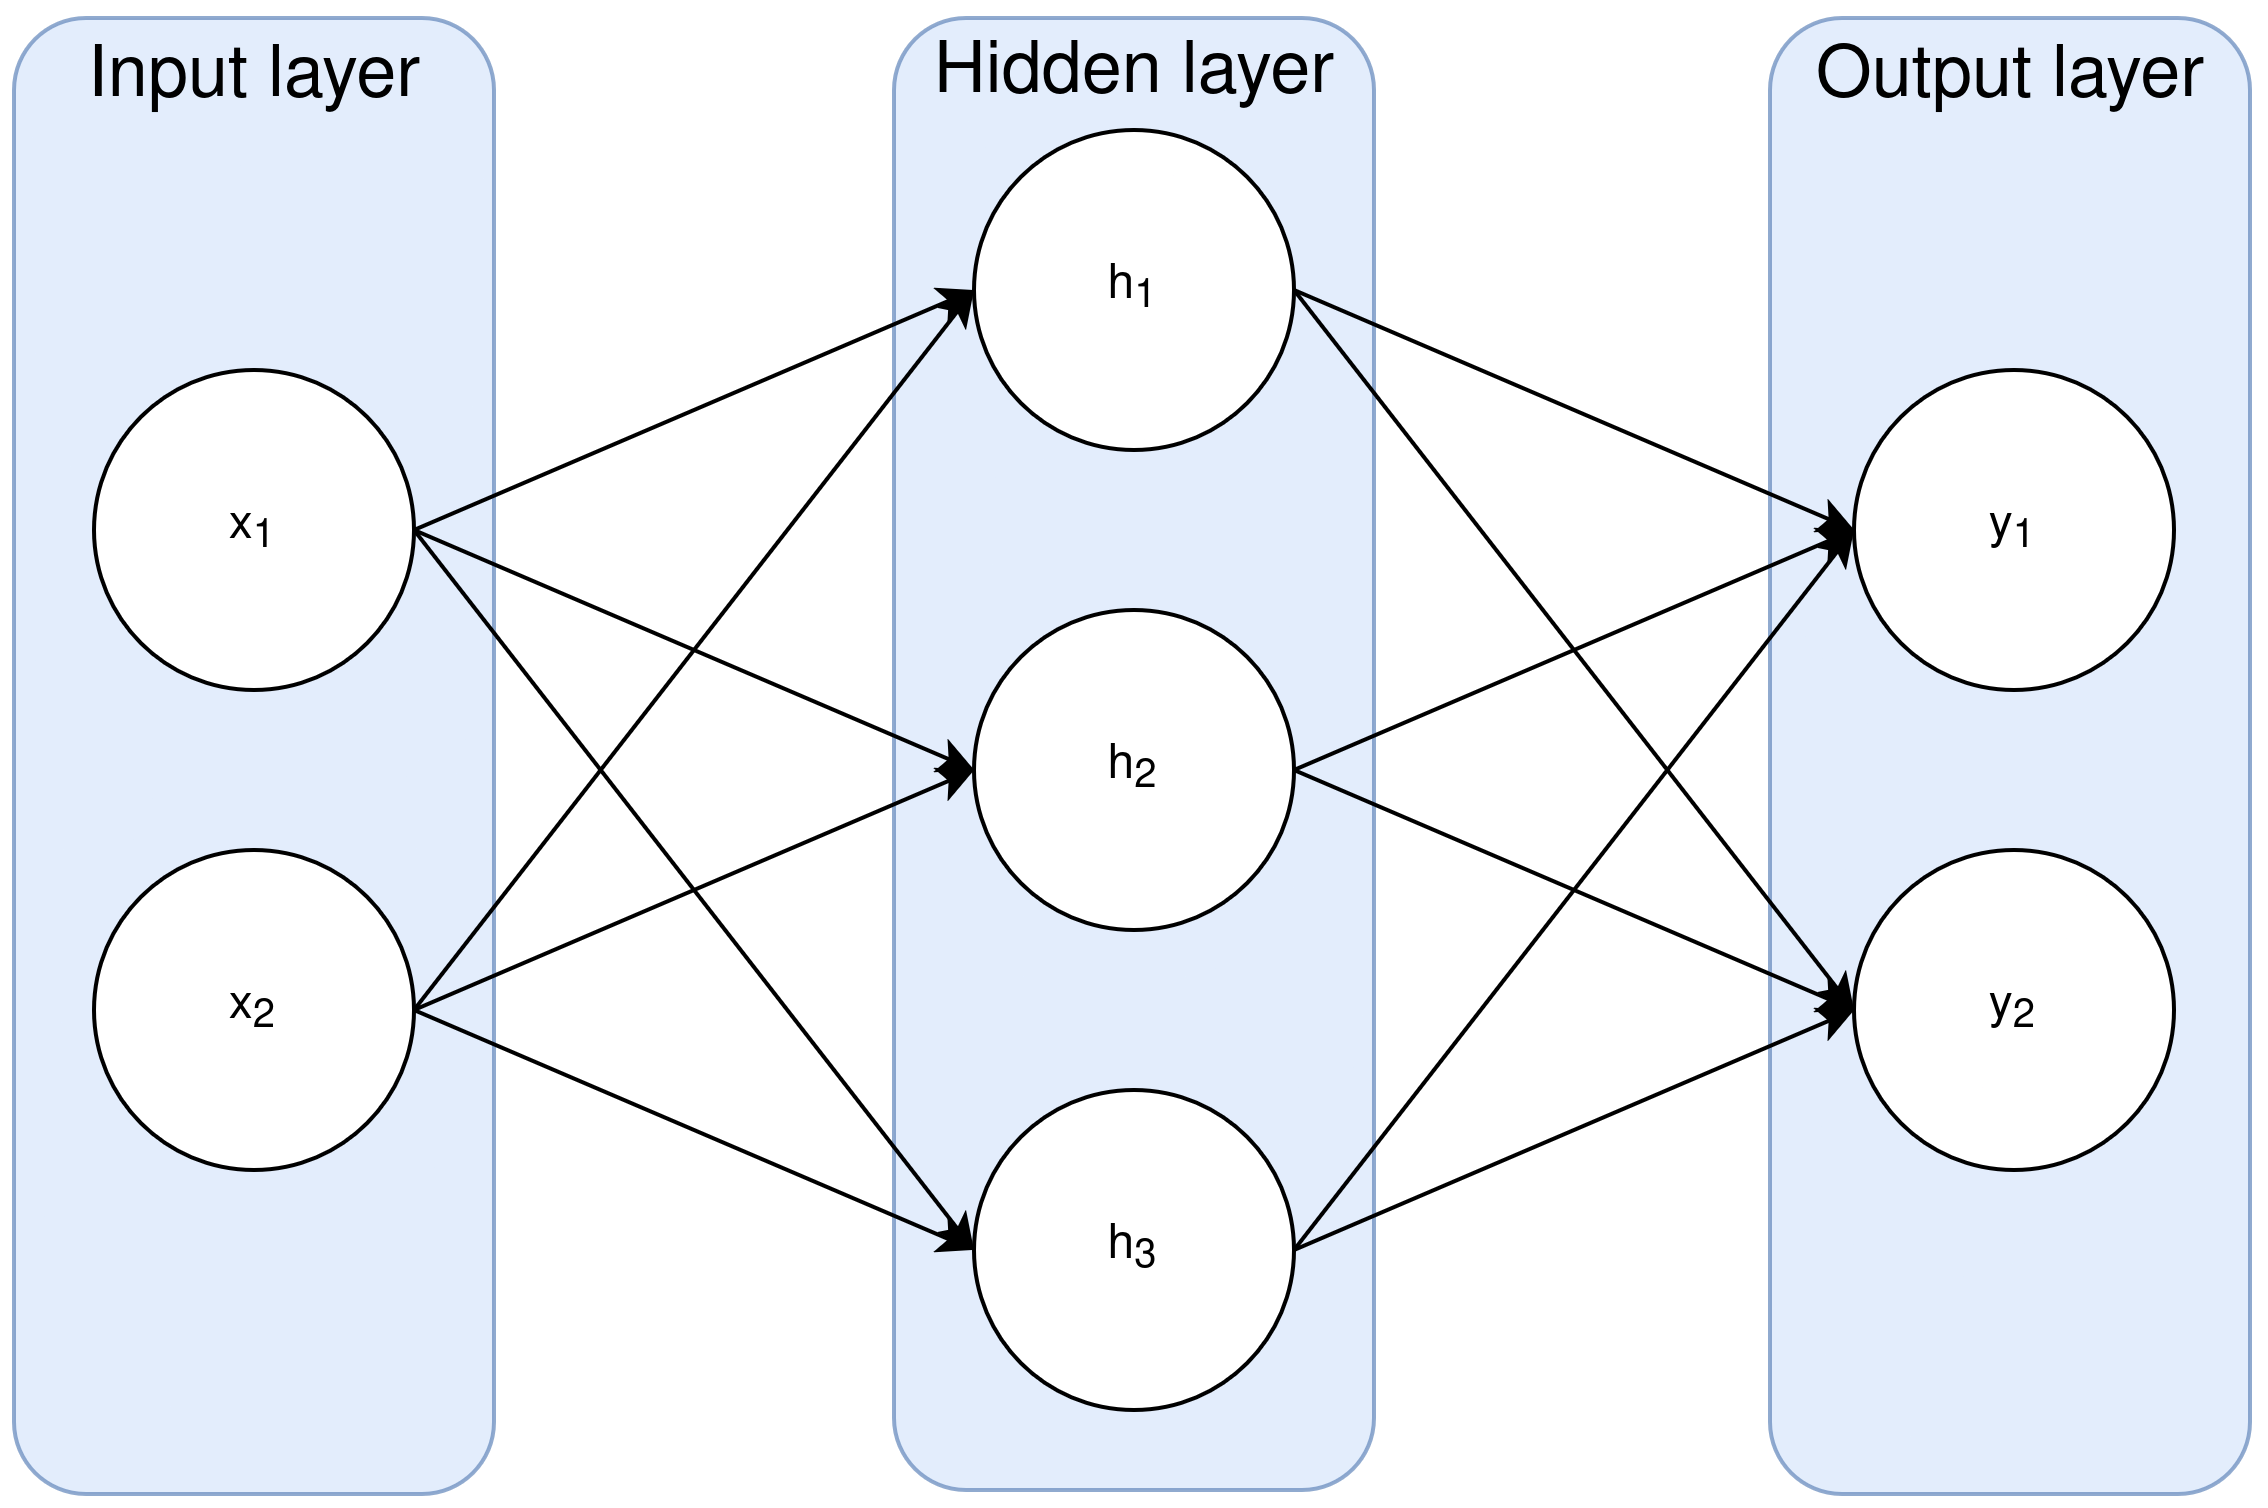
\includegraphics[width=0.6\linewidth]{figures/04_transformer/Shallow_NN.png}
    \caption{Visualization of a feedforward neural network with a single hidden layer containing three neurons, two inputs, and two outputs. The network is fully connected, meaning every unit in one layer is connected to every unit in the next. This is also referred to as a multilayer perceptron. }
\label{fig:shallow_NN}
\end{figure}

Figure~\ref{fig:shallow_NN} shows a shallow feedforward neural network, i.e., one with only a single hidden layer. In a fully connected layer, each neuron is connected to every neuron in the adjacent layers. Although fully connected layers are standard in MLPs, alternative connection patterns exist. 
The first layer is the input layer, the last is the output layer, and all intermediate layers are referred to as hidden layers~\cite{prince_understanding_2023}. In the figure, the hidden layer consists of three computational units, commonly referred to as neurons. 

The computation of a hidden layer is shown in equation~\refeq{eq:NN_hiddenlayer}, where $\mathbf{x} \in \mathbb{R}^d$ is the input vector, $\mathbf{W}_{\theta} \in \mathbb{R}^{m \times d}$ the weight matrix and $\mathbf{b}_{\theta} \in \mathbb{R}^m$ is the bias vector. The non-linear activation function $F$ is applied element-wise. 
The pre-activation (linear part) is given by $\mathbf{W}_{\boldsymbol{\theta}} \cdot \mathbf{x} + \mathbf{b}_{\boldsymbol{\theta}}$, and the activation function transforms it into the hidden representation $\mathbf{h}$. 

An alternative form uses the augmented weight matrix $\mathbf{W'}_{\boldsymbol{\theta}}$ and augmented input $\mathbf{x'}$ to absorb the bias term: 

\begin{align}
\label{eq:NN_hiddenlayer}
	\mathbf{h} & = F \left[ \mathbf{b}_{\theta} + \mathbf{W}_{\theta} \cdot \mathbf{x} \right] = F \left[ \mathbf{W'}_{\theta} \cdot \mathbf{x'} \right] \,,\\
\label{eq:NN_hiddenlayer_out}
	\mathbf{y} & = \mathbf{b}_{\vartheta} + \mathbf{W}_{\vartheta} \cdot \mathbf{h} = \mathbf{W'}_{\vartheta} \cdot \mathbf{h'} \,.
\end{align}

\noindent where $\mathbf{h}$ is the hidden layer. The final output $\mathbf{y}$ is typically a linear transformation of the last hidden layer, optionally followed by an output activation depending on the task. 

While the transformations used in neural networks are commonly referred to as linear layers, they are affine transformations. The inclusion of a bias term makes them not strictly linear in the mathematical sense. However, this can be reformulated as a purely linear operation by augmenting the input vector and weight matrix. Specifically, by extending the input as 

\begin{equation}
\label{eq:affine_to_linear_x}
    \mathbf{x'} = \begin{pmatrix} \mathbf{x} \\ 1 \end{pmatrix} \,,
\end{equation}

\noindent and defining the corresponding augmented weight matrix as

\begin{equation}
\label{eq:affine_to_linear_W}
	\mathbf{W'} = 
	\begin{pmatrix} \mathbf{W} & \mathbf{b}\\
	\mathbf{0}^{\intercal} & 1 \end{pmatrix} \,.
\end{equation}

This trick is widely used in machine learning to streamline notation and implementation, and as such, the bias term is often implied rather than explicitly written. The use of this augmented formulation also clarifies why these layers are often referred to as linear, even though they technically are not. 


\subsubsection{Activation functions}

Historically, the original perceptron used the Heaviside step function as its activation function~\cite{mitchell_machine_1997}. However, modern neural networks typically employ smooth, non-linear, and almost everywhere differentiable activation functions, which enable both more expressive modeling and efficient optimization via gradient-based methods~\cite{murphy_probabilistic_2022}. 
The non-linearity introduced by the activation function is essential. Without it, no matter how many layers are stacked, the overall mapping would collapse to a single affine transformation. Differentiability, on the other hand, is crucial for computing gradients during training. 
It is a remarkable theoretical result that a MLP with just a single hidden layer (given enough hidden units) can approximate any continuous function on a compact domain to arbitrary precision~\cite{hornik_multilayer_1989}. While this universal approximation property is foundational, in practice, deep networks tend to outperform shallow ones; they can more efficiently capture hierarchical or compositional structure, often requiring exponentially fewer units than shallow counterparts to represent the same function class \cite{murphy_probabilistic_2022, telgarsky_2016}.


One of the most widely used activation functions today is the Rectified Linear Unit (ReLU), defined as:

\begin{equation}
\label{eq:ReLU}
	\mathrm{ReLU}(x) = \max(x,0) \,.
\end{equation}

ReLU introduces sparsity by setting all negative inputs to zero while leaving positive values unchanged~\cite{lecun_efficient_2012, Nair_2010, Krizhevsky_2012}. 
A more recent alternative is the Gaussian Error Linear Unit (GELU), a smooth activation function with a non-zero gradient everywhere, which can be advantageous in certain Transformer training setups. Its approximate form is given by:

\begin{equation}
\label{eq:GELU}
	\mathrm{GELU}(x) = \frac{x}{2} \left[ 1 + \mathrm{erf} \left( \frac{x}{\sqrt{2}} \right) \right] \,.
\end{equation}

Unlike ReLU, GELU is smooth and differentiable everywhere, which can improve convergence in deeper networks. GELU is used as the default activation function in many Transformer-based architectures -- deep learning models designed for sequential data processing~\cite{hendrycks_gaussian_2023}. Common activation functions are shown in figure~\ref{fig:Activation_functions}. 

\begin{figure}
    \centering
    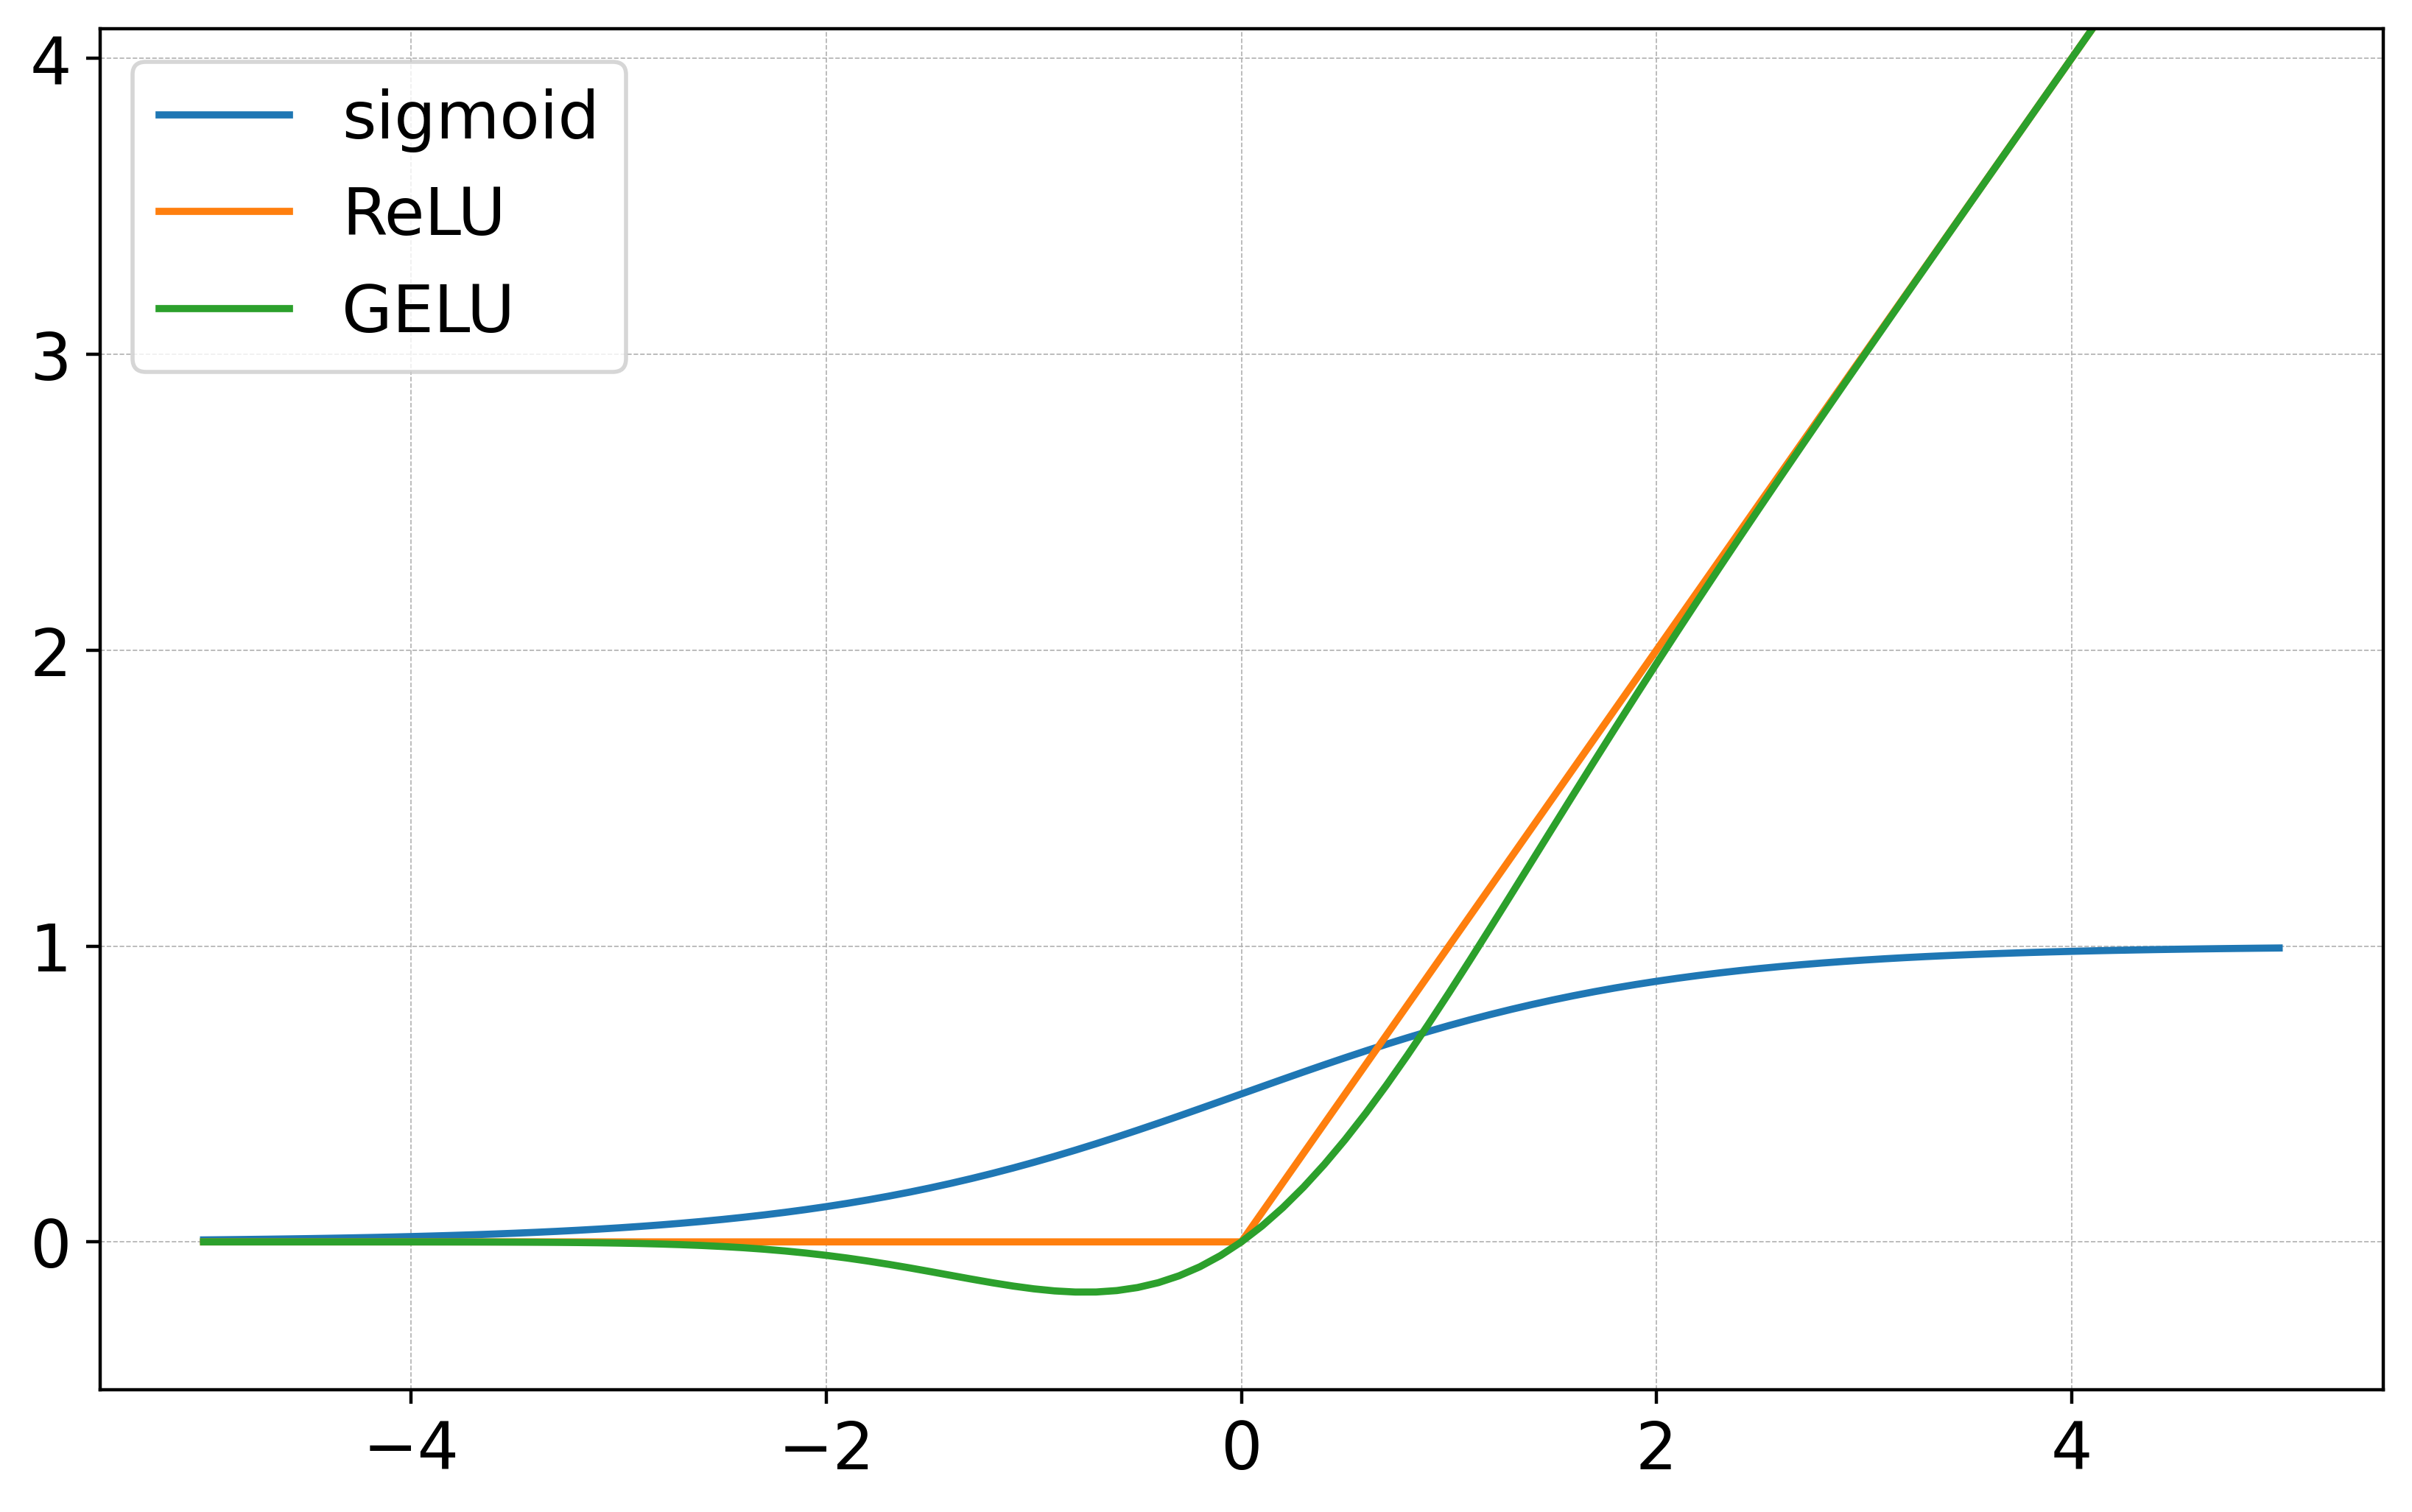
\includegraphics[width=0.7\linewidth]{figures/04_transformer/Activation_functions.png}
    \caption{Common activation functions applied to inputs in the range $x \in [-5, 5]$.}
\label{fig:Activation_functions}
\end{figure}


\subsection{Optimization}
\label{sec:03_optimization}

As seen in the case of linear regression, machine learning aims to determine the optimal parameters $\hat{\boldsymbol{\theta}}$ that describe the mapping $f(\mathbf{x}; \boldsymbol{\theta})$ given a set of input-output pairs $\{\mathbf{x}_i, \mathbf{y}_i\}$. To do so, one minimizes a loss function, a quantitative measure for the discrepancy between the model's predictions and the true target values~\cite{prince_understanding_2023}.  

One of the most widely used principles for parameter estimation is maximum likelihood estimation (MLE). In this approach, we seek the parameters ${\boldsymbol{\theta}} \in \mathcal{T}$ that maximize the likelihood of the data given the parameters. Assuming that the training samples are drawn independently from the same distribution, the likelihood function factorizes, and the MLE takes the form:
\begin{equation}
\label{eq:maximum_likelihood}
    \hat{\boldsymbol{\theta}} = \underset{\boldsymbol{\theta}}{\mathrm{argmax}} \; P\left( \mathcal{T} \mid \boldsymbol{\theta} \right) = \underset{\boldsymbol{\theta}}{\mathrm{argmax}} \prod_{i=1}^N P\left( \mathbf{y}_i \mid \mathbf{x}_i; \boldsymbol{\theta} \right)\,.
\end{equation}

In practice, working with products of probabilities is numerically unstable and analytically inconvenient. Instead, it is customary to use the negative log-likelihood (NLL) as a loss function, which transforms the product into a sum: 

\begin{equation}
\label{eq:neg_log_likelihood}
	\hat{\boldsymbol{{\theta}}} = \underset{\boldsymbol{\theta}}{\mathrm{argmin}} \; \mathrm{NLL}\left( \boldsymbol{\theta} \right) = \underset{\boldsymbol{\theta}}{\mathrm{argmin}} \; \left[ - \sum_{i=1}^N  \log P \left( \mathbf{y}_i  \mid \mathbf{x}_i; \boldsymbol{\theta} \right) \right] \,.
\end{equation}

This formulation is widely used across regression and classification tasks. In fact, the least-squares loss introduced in equation~\refeq{eq:least_squares} is a special case of equation~\refeq{eq:neg_log_likelihood}, where we assume a Gaussian likelihood with a fixed variance~\cite{murphy_probabilistic_2022, zhang_dive_2023}.


A widely used loss function in supervised classification tasks is the cross-entropy loss, which measures the dissimilarity between the empirical distribution $q(y)$ of the observed data and the predicted distribution $p(y)$ of the model. Minimizing cross-entropy is equivalent to minimizing the Kullback-Leibler divergence between the true and predicted distributions when the true distribution is fixed~\cite{prince_understanding_2023}. The cross-entropy is defined as:

\begin{equation}
\label{eq:cross_entropy}
	\mathbb{H}(q,p) = - \sum_y q(y) \log{p(y)} \,.
\end{equation}

In classification settings, the true distribution $q(y)$ is often represented as a one-hot vector, where the entry corresponding to the correct class is 1 and all others are 0. The predicted distribution $p(y)$ is typically the output of a softmax function applied to the final layer of the network. 
However, cross-entropy loss may perform poorly when the dataset is class-imbalanced, as the model is biased toward majority classes. To address this, the focal loss was introduced~\cite{lin_focal_2018}. It extends the cross-entropy by a modulating factor $(1 - p_t)^{\gamma}$, where $p_t$ is the model's predicted probability for the true class. This factor down-weights well-classified examples and focuses learning on hard, misclassified instances~\cite{lin_focal_2018}:

\begin{equation}
\label{eq:focal_loss}
	L_{\mathrm{focal}} \left( \mathbf{y}, \hat{\mathbf{p}} \right)  = - \left( 1 - \hat{p_y} \right)^{\gamma} \, \log \hat{p_y} \,.
\end{equation}

Here, $\mathbf{y}$ is the true class label (as an integer) and $\hat{\mathbf{p}}$ is a vector representing an estimated probability distribution over the classes~\cite{mavrin_artemmavrinfocal-loss_2024}. 

Another loss function commonly used in imbalanced classification problems is the Dice loss, derived from the Dice-Sørensen coefficient. It measures the overlap between predicted and true class distributions and is especially useful in segmentation tasks with extreme class imbalance, such as in medical imaging. The multi-class Dice loss is given by:

\begin{equation}
\label{eq:dice_score}
	L_{\mathrm{Dice}} = 1 - \frac{1}{N_c} \sum_{i=1}^{N_c} \frac{2 y_i \hat{p}_i + \epsilon}{y_i + \hat{p}_i + \epsilon} \,,
\end{equation}

\noindent where $\mathbf{y}, \hat{\mathbf{p}} \in \mathbb{R}^{N_c}$ represent the true and predicted class probabilities, respectively, and $\epsilon$ is a small factor to ensure this function is always well-defined. It is possible to combine different loss functions, for example, by defining a combined loss as the sum of Dice and focal loss:

\begin{equation}
\label{eq:combined_loss}
	L_{\mathrm{combined}} = L_{\mathrm{focal}} + L_{\mathrm{Dice}} \,.
\end{equation}

Taghanaki et al. showed that a weighted sum of Dice and focal loss outperforms other state-of-the-art methods in medical imaging analysis~\cite{taghanaki_combo_2019}.  



\subsubsection{Optimization algorithms}
\label{sec:03_optimization_algorithms}

Various optimization algorithms are available for minimizing the loss function, but the most fundamental is gradient descent. It works as follows: 
At each iteration $i$, the gradient of the loss with respect to the parameters is computed (equation~\refeq{eq:gradient_descent1}), and the parameters are then updated by a step of size $\alpha$ (the learning rate):

\begin{align}
\label{eq:gradient_descent1}
	\grad L & = \frac{\partial L}{\partial \theta} \,,\\
\label{eq:gradient_descent2}
	\theta_{i+1} & = \theta_i - \alpha \cdot \grad L \,.
\end{align}

When the gradient approaches zero, successive updates become negligible. In practice, most algorithms terminate if the change in parameters falls below a predefined threshold~\cite{prince_understanding_2023}.
It can be very challenging to optimize loss functions using gradient descent. If the learning rate is too small, convergence is slow, and if it's too large, the algorithm may overshoot or diverge. In high-dimensional, non-convex problems such as deep learning, plateaus, saddle points, and poor curvature are problematic~\cite{murphy_probabilistic_2022}. 

Stochastic gradient descent (SGD) reduces the computational cost and helps escape poor regions of the loss function by replacing the full gradient with an expectation over a random subset of the data:

\begin{equation}
\label{eq:stochastic_optimization}
	\mathbb{E}_{q(\mathbf{z})} \left[ L \left( \boldsymbol{\theta}, \mathbf{z} \right) \right] \,.
\end{equation}

Here, $\mathbf{z}$ denotes a mini-batch, and the expectation is taken over the empirical data distribution $q(\mathbf{z})$, which is typically approximated as uniform over the available training samples. The inherent noise introduced by this stochastic sampling not only reduces computation but also improves generalization by preventing the model from settling into sharp or narrow local minima that might overfit the training data~\cite{prince_understanding_2023}. 
Computing the gradient over a batch $\mathcal{B}$ of size $\|\mathcal{B}\|$ gives: 

\begin{equation}
\label{eq:batch_stochastic_gradient_descent}
	\grad L_{\mathcal{B}} = \frac{\partial}{\partial  \boldsymbol{\theta}} \frac{1}{\|\mathcal{B}\|} \sum_{i \in \mathcal{B}} L(\mathbf{x}_i, \boldsymbol{\theta}) \,.
\end{equation}

This notably reduces gradient variance compared to single-sample updates~\cite{zhang_dive_2023}.
Momentum incorporates a running average of past gradients. Instead of moving purely in the direction of the current gradient, the update accumulates a velocity term that reflects recent gradient history. 
This approach dampens oscillations in noisy directions and accelerates along shallow but consistent slopes. Momentum often leads to faster convergence and better traversal of narrow valleys in the loss landscape~\cite{zhang_dive_2023, murphy_probabilistic_2022}. 
Defining: 

\begin{equation}
\label{eq:momentum1}
	m_{i+1} = \beta \cdot m_i + \grad L \,.
\end{equation}

The parameters are updated via

\begin{equation}
\label{eq:momentum2}
	\theta_{i+1} = \theta_i - \alpha \cdot m_{i+1} \,,
\end{equation}

\noindent where $\beta$ is the momentum coefficient, typically $\sim 0.9$, that controls the contribution of past gradients. 

The Adaptive Moment Estimation (Adam) optimizer combines stochastic optimization and momentum~\cite{kingma_adam_2017}. For this, we define:

\begin{align}
\label{eq:ADAM1}
	\tilde m_{i+1} & = \beta_1 \cdot \tilde m_i + (1 - \beta_1) \grad L \,,\\
\label{eq:ADAM2}
	\tilde s_{i+1} & = \beta_2 \cdot \tilde s_i + (1 - \beta_2) \left(\grad L \right)^2 \,,
\end{align}

\noindent where $\tilde m_i$ is the normalized momentum and $\tilde s_i$ is the normalized second moment of the gradient. The normalization is to avoid bias at the beginning of the training, where only a few past gradients exist. It is given as $\tilde m_i = \frac{m_i}{(1 - \beta_1)}$ and analogous for $\tilde s_i$. 
The parameters are updated as follows: 

\begin{equation}
\label{eq:ADAM3}
\theta_{i+1} = \theta_i - \alpha \frac{\tilde m_i}{\sqrt{\tilde s_i} + \epsilon} \,,
\end{equation}

\noindent where $\alpha$ is the learning rate and $\epsilon$ is a small constant to avoid division by zero. The standard values are $\beta_1 = 0.9$, $\beta_2 = 0.999$, and $\epsilon = 10^{-6}$~\cite{murphy_probabilistic_2022}. Figure~\ref{fig:Optimization_plots} shows the implementation of SGD, momentum, and Adam on an ill-conditioned quadratic loss surface, $L(\boldsymbol{\theta}) = \frac{1}{2} \left( 1 \cdot {\theta^{(0)}}^2 + 0.5 \cdot {\theta^{(1)}}^2 \right)$.

\begin{figure}
    \centering
    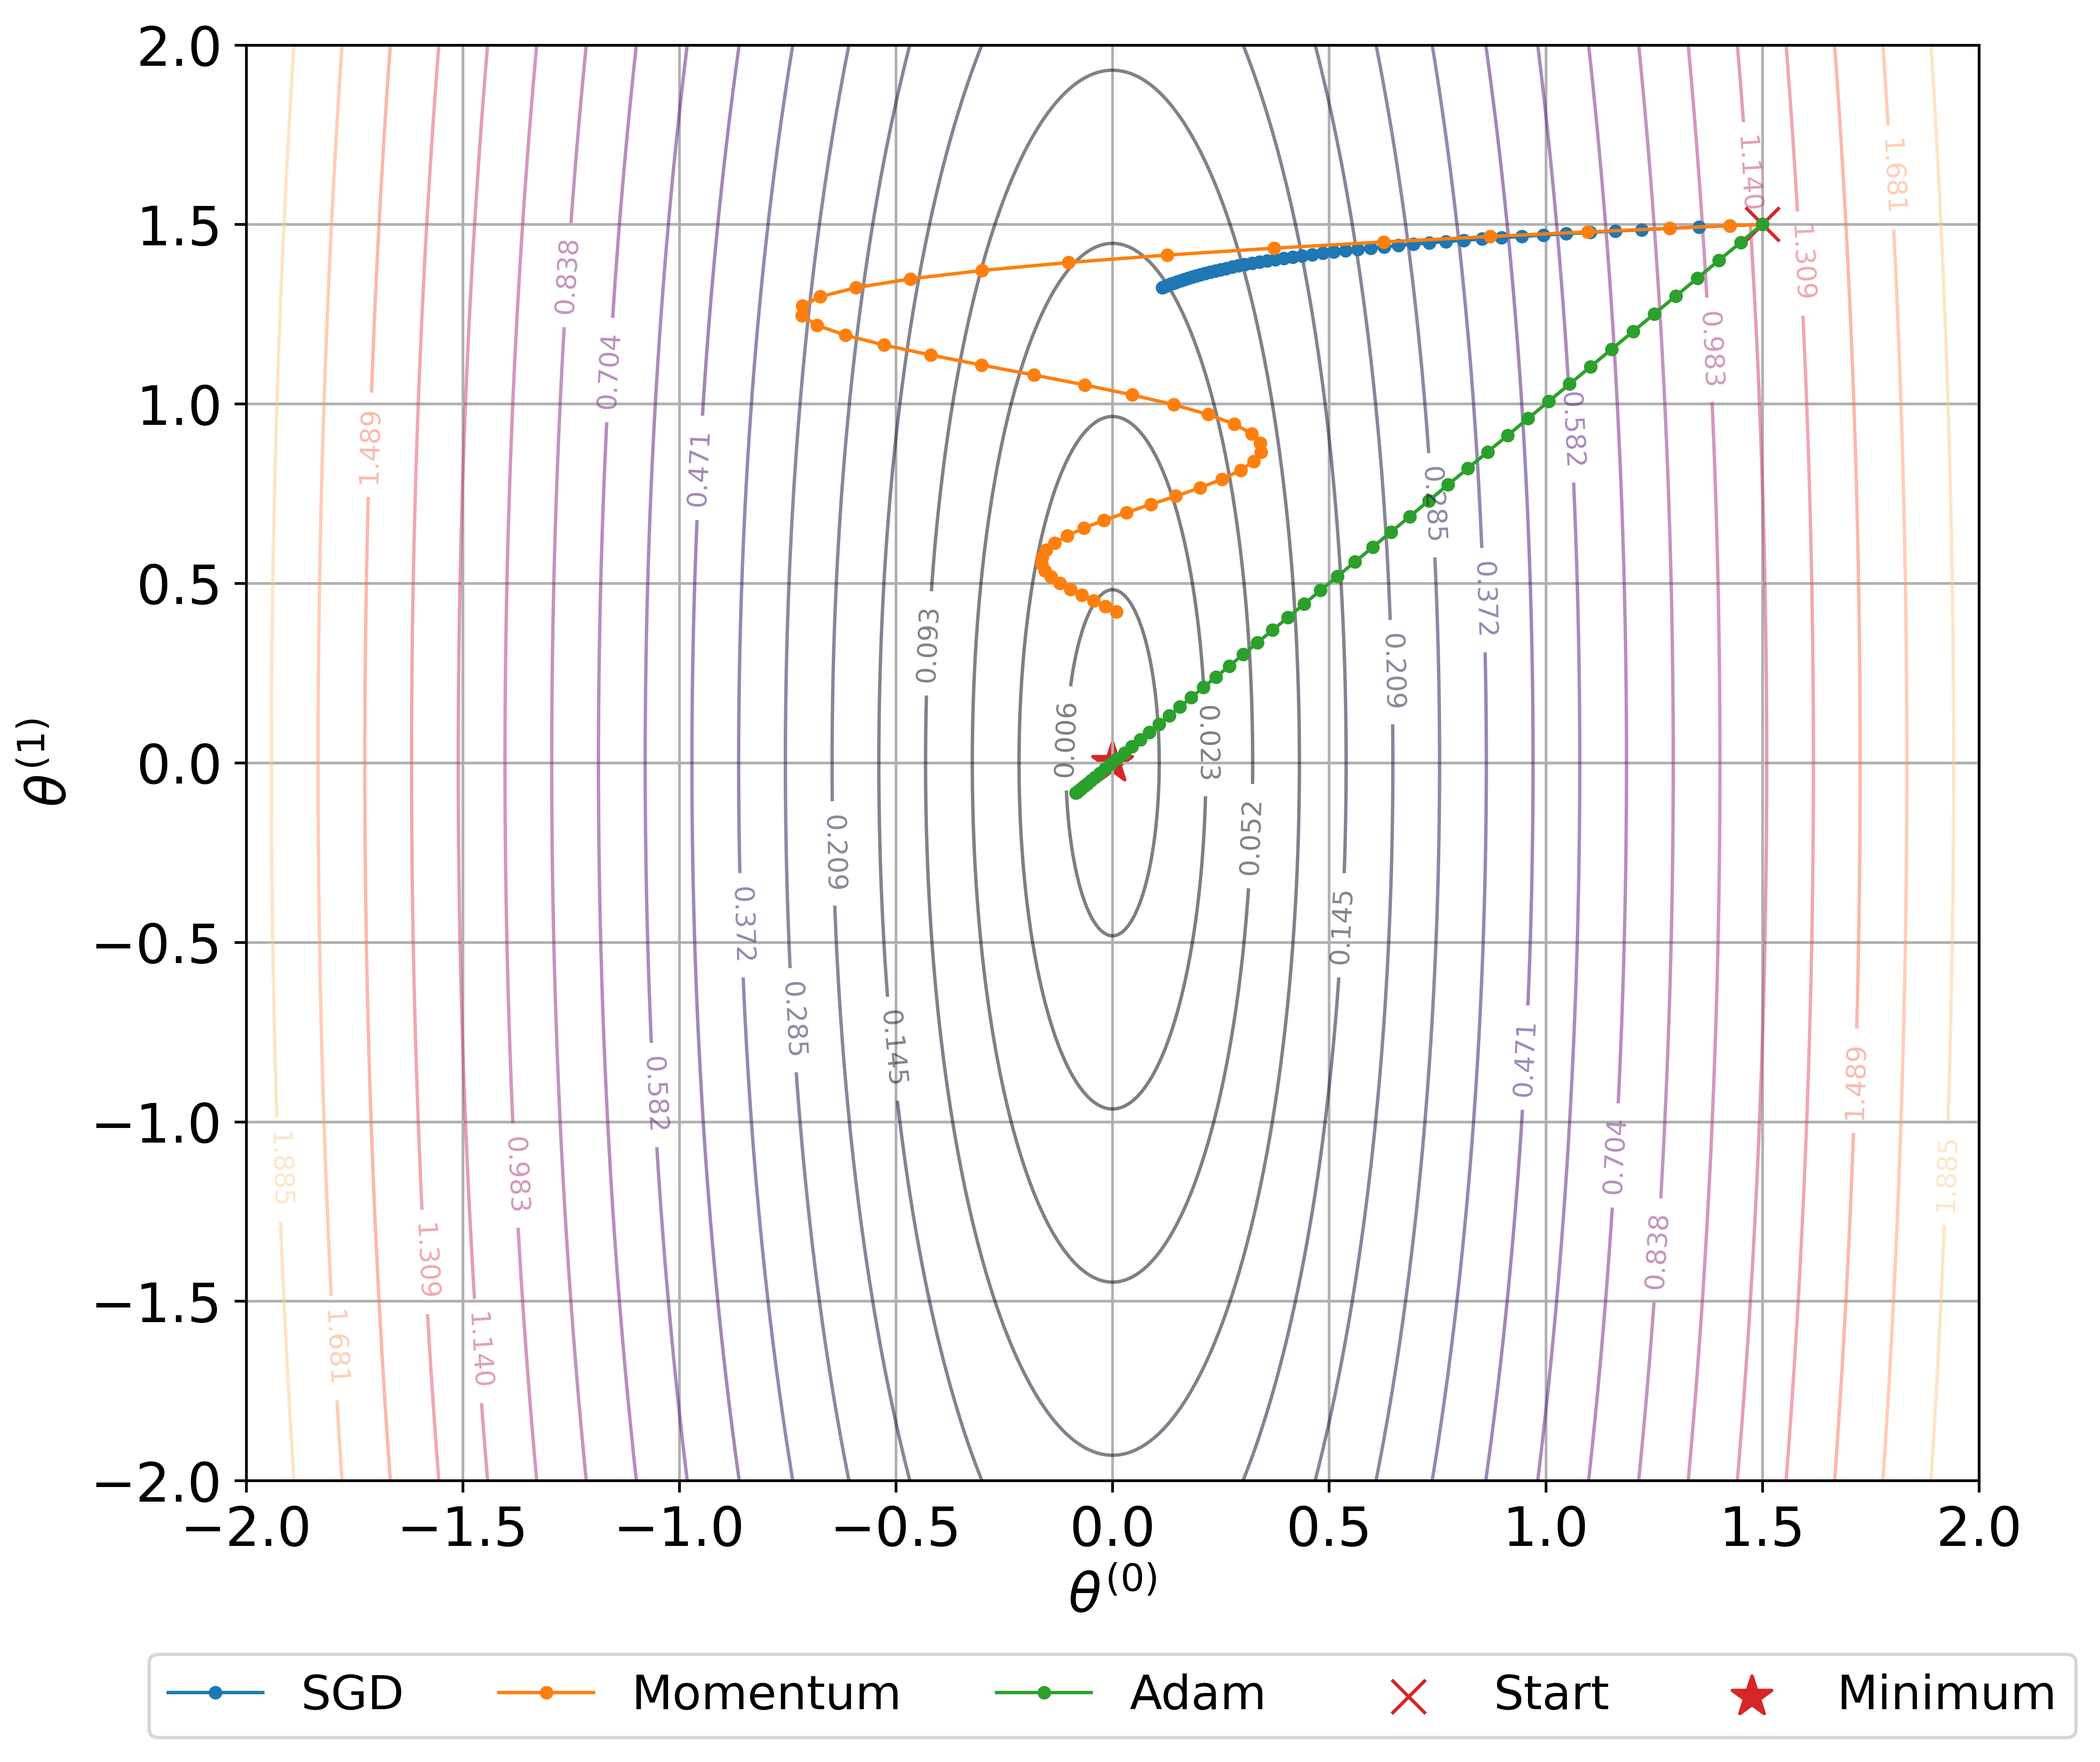
\includegraphics[width=0.85\linewidth]{figures/04_transformer/Transformer_optimization.png}
    \caption{Optimizer trajectories on an ill-conditioned quadratic loss surface, illustrating the behavior of SGD, momentum ($\beta = 0.9$) and Adam ($\beta_1 = 0.9, \; \beta_2 = 0.999$). The horizontal and vertical axes correspond to the two components of the parameter vector; colors show the loss value. SGD follows a slow path down the valley before curving toward the minimum, momentum overshoots and oscillates along the narrow direction before converging, and Adam adapts the step sizes to move almost directly toward the minimum. The number of iterations is set to 40, and the learning rate is set to $\alpha = 0.05$ for all algorithms.}
\label{fig:Optimization_plots}
\end{figure}

\subsubsection{Backpropagation}

As described in Section~\ref{sec:03_optimization_algorithms}, optimization requires calculating the gradients of the loss functions with respect to every trainable parameter in the model. In deep neural networks, the number of parameters can be in the millions. It is therefore important to compute these gradients efficiently~\cite{prince_understanding_2023}. This is the role of the well-known backpropagation algorithm. 

Let us consider the shallow neural network shown in  figure~\ref{fig:shallow_NN}, which consists of a single hidden layer. The network's operations during a forward pass can be described by the following sequence of functions:

\begin{align}
\label{eq:backprop_example_forwardpass}
	x_2 & = f_1(x; \theta_1) & \text{(linear combination)} \\ 
	x_3 & = f_2(x_2) & \text{(activation)} \\
	x_4 & = f_3(x_3; \theta_3) & \text{(linear combination)} \\
	L & = f_4(x_4, y) & \text{(loss)} 
\end{align}

\begin{figure}
    \centering
    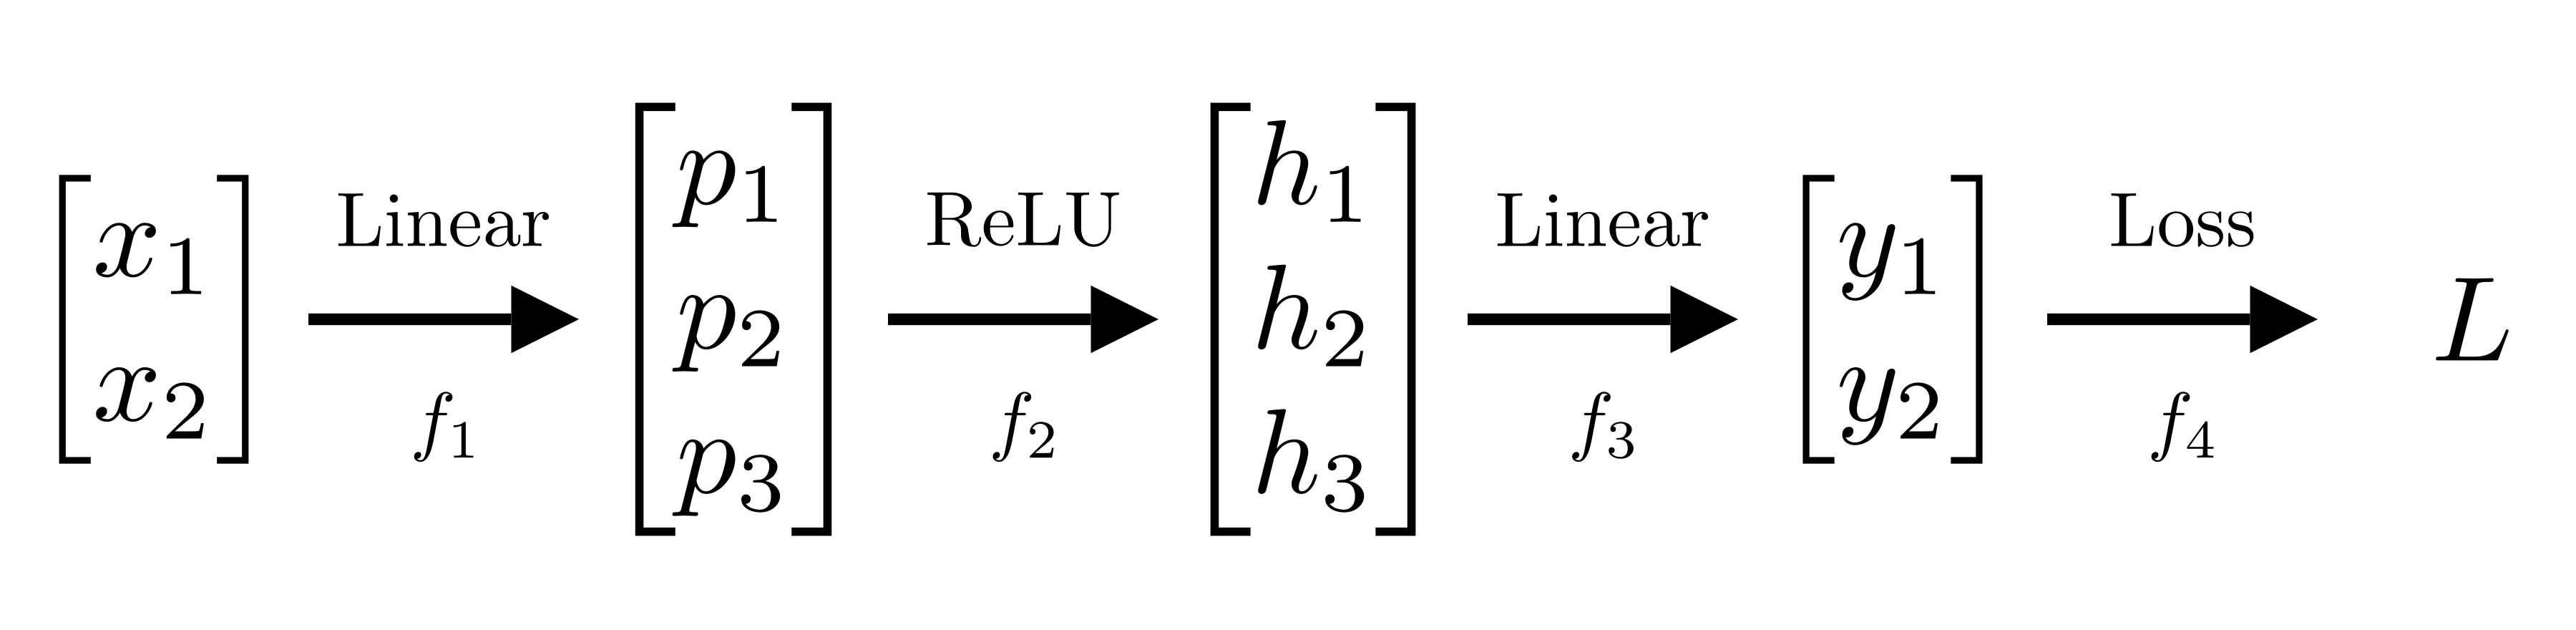
\includegraphics[width=0.85\linewidth]{figures/04_transformer/Shallow_NN_operations.png}
    \caption{Visualization of the MLP in figure~\ref{fig:shallow_NN}, where each operation is displayed separately. The hidden layer is split into pre-activation and activation. Plot created with~\cite{the_manim_community_developers_manim_2025}.}
\label{fig:shallow_NN_operation}
\end{figure}


\noindent Here, $x$ and $y$ are the input and true output, respectively. The network as a whole can be written as the composition $f = f_4 \circ f_3 \circ f_2 \circ f_1$. This is illustrated in figure~\ref{fig:shallow_NN_operation}. Note that the activation function $f_2$ has no trainable parameters, as it only introduces a non-linearity. 

Already small changes to parameters can be amplified as they propagate through the network. To compute how a change in a parameter, such as $\theta_3$ affects the loss, we need to know how intermediate quantities like $x_4$ respond. 
For a parameter further away from the output, such as $\theta_1$, the influence must be computed through a chain of dependencies: From $x_2$ to $x_3$, from $x_3$ to $x_4$, and finally from $x_4$ to the loss. 
The backpropagation algorithm exploits this structure: Rather than recomputing gradients from scratch at every layer, it reuses intermediate results. This leads to significant computational savings. The backward pass proceeds from the output layer back toward the input:

\begin{align}
\label{eq:backprop_example_backwardpass}
	\frac{\partial L}{\partial \theta_3} & = \frac{\partial L}{\partial x_4} \frac{\partial x_4}{\partial \theta_3} \,,\\
	\frac{\partial L}{\partial \theta_1} & = \frac{\partial L}{\partial x_4} \frac{\partial x_4}{\partial x_3} \frac{\partial x_3}{\partial x_2} \frac{\partial x_2}{\partial \theta_1} \,.
\end{align}

Each $\frac{\partial L}{\partial \theta_k}$ is a row vector that can be computed recursively by propagating the upstream gradient through the network. Specifically, it is obtained by multiplying the gradient from the previous layer of the Jacobian $\frac{\partial x_k}{\partial x_{k-1}}$, which captures how changes in the input layer $k -1$ affect the output of layer $k$. This recursive structure enables efficient computations of gradients.
The Jacobian matrix itself is defined as:


\begin{equation}
\label{eq:backprop_jacobian}
	\mathbf{J_f} =  
\begin{pmatrix} 
\frac{\partial f_1}{\partial x_1} & \cdots & \frac{\partial f_1}{\partial x_n} \\
\vdots & \ddots & \vdots \\
\frac{\partial f_m}{\partial x_1} & \cdots &  \frac{\partial f_m}{\partial x_n} \\
\end{pmatrix} 
	= \begin{pmatrix} \grad f_1 (\mathbf{x})^{\intercal} \\ \vdots \\ \grad f_m(\mathbf{x})^{\intercal} \end{pmatrix}
	= \begin{pmatrix} \frac{\partial \mathbf{f}}{\partial x_1 } \ldots \frac{\partial \mathbf{f}}{\partial x_n}\end{pmatrix} \in \mathbb{R}^{m \times n} \,.
\end{equation}

Depending on the dimensions of the input $n$ and output $m$, the Jacobian is calculated differently. If $n < m$, it is more efficient to calculate each row $\frac{\partial \mathbf{f}}{\partial x_j}$. 
However, in practice, scalar outputs are common ($m = 1$), making it more efficient to compute the Jacobian columns $\grad f_i(x)^{\intercal}$. 

The backward algorithm then proceeds recursively, starting from $u_{K+1}^{\intercal} = 1$ and iterating $k$ from $K$ to 1:

\begin{align}
\label{eq:backprop_backwardpass}
	g_k & = u_{k+1}^{\intercal} \frac{\partial \mathbf{f}_k(x_k, \theta_k)}{\partial \theta_k} \,,\\
	u_k^{\intercal} & = u_{k+1}^{\intercal} \frac{\partial \mathbf{f}_k(x_k, \theta_k)}{\partial x_k} \,. 
\end{align}

This algorithm is computationally very efficient, as the most expensive operations are matrix multiplications, which can be parallelized and executed rapidly on modern hardware. 


\subsubsection{Traning stability}
Despite the efficiency of the backpropagation algorithm, training large neural networks remains challenging. During backpropagation, gradients are computed using the chain rule and propagated recursively through each layer.
However, if these derivatives are small, their repeated multiplication can lead to vanishing gradients, where gradients become too small to update parameters effectively. Similarly, very large derivatives can result in exploding gradients, where parameters become unstable. 
The latter can be controlled using gradient clipping, where gradients exceeding a certain threshold $c$ are scaled down~\cite{murphy_probabilistic_2022}:

\begin{equation}
\label{eq:gradient_clipping}
    \mathbf{g}' = \min(1, \frac{c}{\norm{\mathbf{g}}}) \, \mathbf{g} \,,
\end{equation}

\noindent where $\mathbf{g}'$ is the scaled gradient that goes in the same direction as the gradient $\mathbf{g}$.


The vanishing gradient can be mitigated by using a loss function whose gradient is not too small, which is the case for ReLU and GELU.  
An effective approach is the use of residual connections, illustrated in figure~\ref{fig:ResidualMLP}. In a residual network, each perceptron computes:

\begin{equation}
\label{eq:residual_layer}
	\mathcal{F'}(x) = \mathcal{F}(x) + x\,,
\end{equation}

\noindent where $\mathcal{F}(x)$ is the standard non-linear transformation (e.g., a layer or network), as defined earlier in equation~\refeq{eq:NN_hiddenlayer}~\cite{he_deep_2015}. While this does not increase the number of trainable parameters, it improves trainability~\cite{murphy_probabilistic_2022}. 
To see this, consider the gradient in the residual case:

\begin{figure}[t]
    \centering
    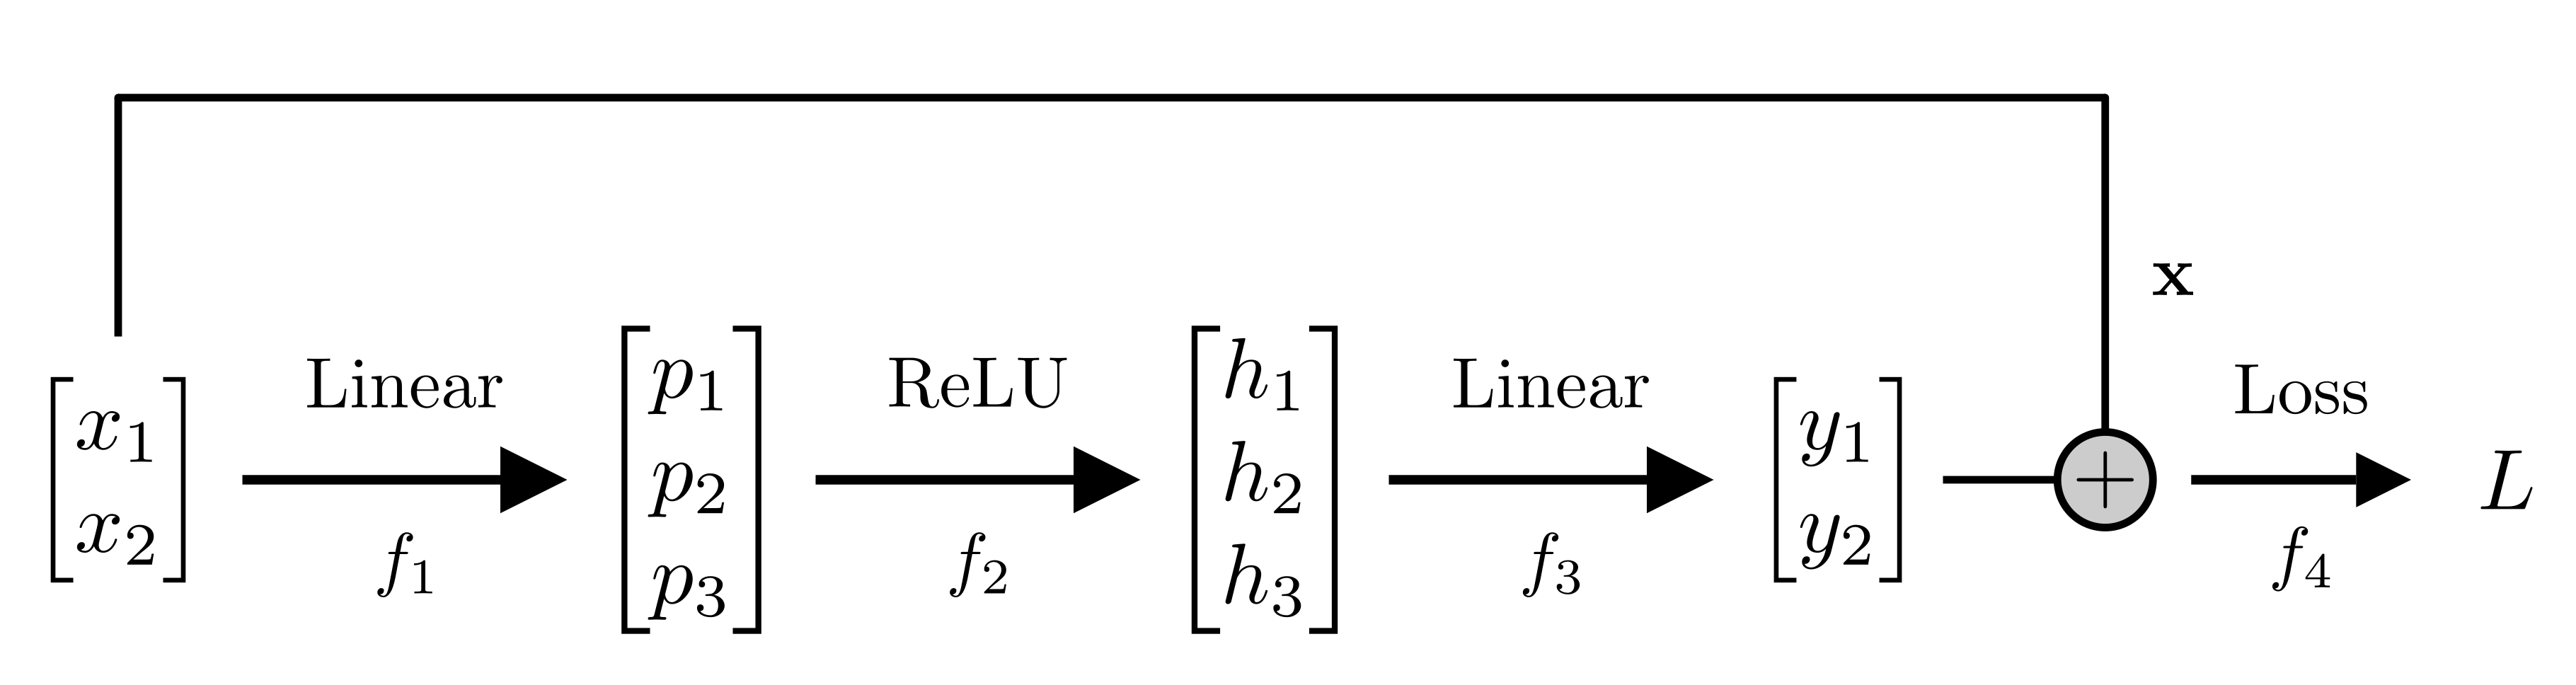
\includegraphics[width=0.95\linewidth]{figures/04_transformer/ResidualMLP.png}
    \caption{Multilayer perceptron of figure~\ref{fig:shallow_NN_operation}, but including a residual connection, which is indicated by the line adding $\mathbf{x}$ to the output $\mathbf{y}$. Plotted with~\cite{the_manim_community_developers_manim_2025}.}
\label{fig:ResidualMLP}
\end{figure}


\begin{equation}
\label{eq:backprop_resnet}
	\frac{\partial L}{\partial \theta_3} = \frac{\partial L}{\partial x_4} \frac{\partial x_4}{\partial x_3} \frac{\partial x_3}{\partial \theta_2} = \frac{\partial L}{\partial x_4} \left( \frac{\partial f_3}{\partial x_3} + \mathbb{1} \right) \frac{\partial x_3}{\partial \theta_2} \,.
\end{equation}

The identity term $\mathbb{1}$ arises because $x_3$ is directly added to $f_3$. Hence even if $\frac{\partial f}{\partial x_3}$ is very small, the gradient will not vanish~\cite{murphy_probabilistic_2022}.

Another key technique to improve numerical stability is normalization. Two commonly used methods are batch normalization and layer normalization. 

Batch normalization standardizes the pre-activations to zero mean and unit variance. Recall that the equation for a hidden unit in a fully connected NN was $h_d = F \left[ \mathbf{b}_\theta + \mathbf{W}_{\theta} \cdot \mathbf{x} \right]$. 
We can add a batch normalization as follows: 

\begin{equation}
\label{eq:NN_hidden_unit_BN}
	h_d = F \left[ \mathrm{BN}(\mathbf{b}_\theta + \mathbf{W}_{\theta} \cdot \mathbf{x}) \right] \,.
\end{equation}

For a given batch $\mathcal{B}$ the batch normalization is defined as:

\begin{equation}
\label{eq:BN_def}
	\mathrm{BN}(\mathbf{x}) = \gamma \circ \frac{\mathbf{x} - \mathbf{\mu_{\mathcal{B}}}}{\mathbf{\sigma_{\mathcal{B}}}} + \beta \,,
\end{equation}

\noindent Here $\mu_{\mathcal{B}}$ and $\sigma_{\mathcal{B}}$ indicate the mean and the standard deviation of the batch, calculated as in equations~\refeq{eq:BN_mean} and~\refeq{eq:BN_std} where $\epsilon$ is again a small parameter (we used $\epsilon = 10^{-5}$) to avoid division by zero.
This introduces two new parameters $\gamma$ and $\beta$ that are learned during training~\cite{zhang_dive_2023, murphy_probabilistic_2022}.

\begin{align}
\label{eq:BN_mean}
	\mu_{\mathcal{B}} & = \frac{1}{\|\mathcal{B}\|} \sum_{x \in \mathcal{B}} \mathbf{x} \,,\\
\label{eq:BN_std}
	\sigma_{\mathcal{B}} & = \sqrt{\frac{1}{\|\mathcal{B}\|} \sum_{x \in \mathcal{B}} \left( x - \mu_{\mathcal{B}} \right)^2 + \epsilon} \;.
\end{align}

Batch normalization works well for large enough batch sizes. Layer normalization is defined similarly. However, the normalization is applied over all the hidden units in a single layer of a single vector $\mathbf{x}$, making it independent of batch size. It works well for recurrent and Transformer-based models because it avoids dependence on batch-level statistics, which may be unstable or poorly defined when working with variable-length sequences or in small batch sizes, common in NL and sequence modelling. The mean and variance are computed as:

\begin{align}
\label{eq:LN_mean}
	\mu_{\mathcal{L}} &  = \frac{1}{H} \sum_{i=1}^{H} x_i \,, \\
\label{eq:LN_std}
	\sigma_{\mathcal{L}}^2 & = \frac{1}{H} \sum_{i=1}^H \left( x_i - \mu_{\mathcal{L}} \right)^2 \,,
\end{align}

\noindent where $H$ is the number of hidden units and $x_i$ refers to the activation of the i-th hidden unit in the current layer. Both $\mu_{\mathcal{L}}$ and $\sigma_{\mathcal{L}}^2$ are scalars. As with batch normalization, learnable scale and shift parameters $\gamma$ and $\beta$ are applied~\cite{zhang_dive_2023, ba_layer_2016}.  



\subsection{The Transformer network}

Although MLPs are very powerful in approximating any function, they are limited in their ability to capture relationships across structured or sequential input. In particular, when the input consists of temporally ordered data such as waveforms, MLPs struggle to model long-range dependencies. This limitation motivates the use of architectures specifically designed for such data structures, such as the Transformer network, which was introduced by Vaswani et al. in 2017~\cite{vaswani_attention_2023}. Unlike previous neural network models for sequential data, the Transformer relies exclusively on attention mechanisms. However, later variants reintroduce these components for efficiency or domain-specific modelling. 
Initially developed for natural language processing, Transformer models have since been successfully adapted to a wide variety of domains. Prominent examples include AlphaFold for protein folding~\cite{madani_large_2023}, DALL-E for image generation~\cite{parmar_image_2018}, and large language models such as ChatGPT~\cite{openai_gpt-4_2024}. 

Transformers typically follow an encoder-decoder structure. However, depending on the specific task, encoder-only or decoder-only architectures are often sufficient. For instance, ChatGPT uses a decoder-only model, whereas the Transformer used in this work relies only on an encoder. 


\begin{figure}
    \centering
    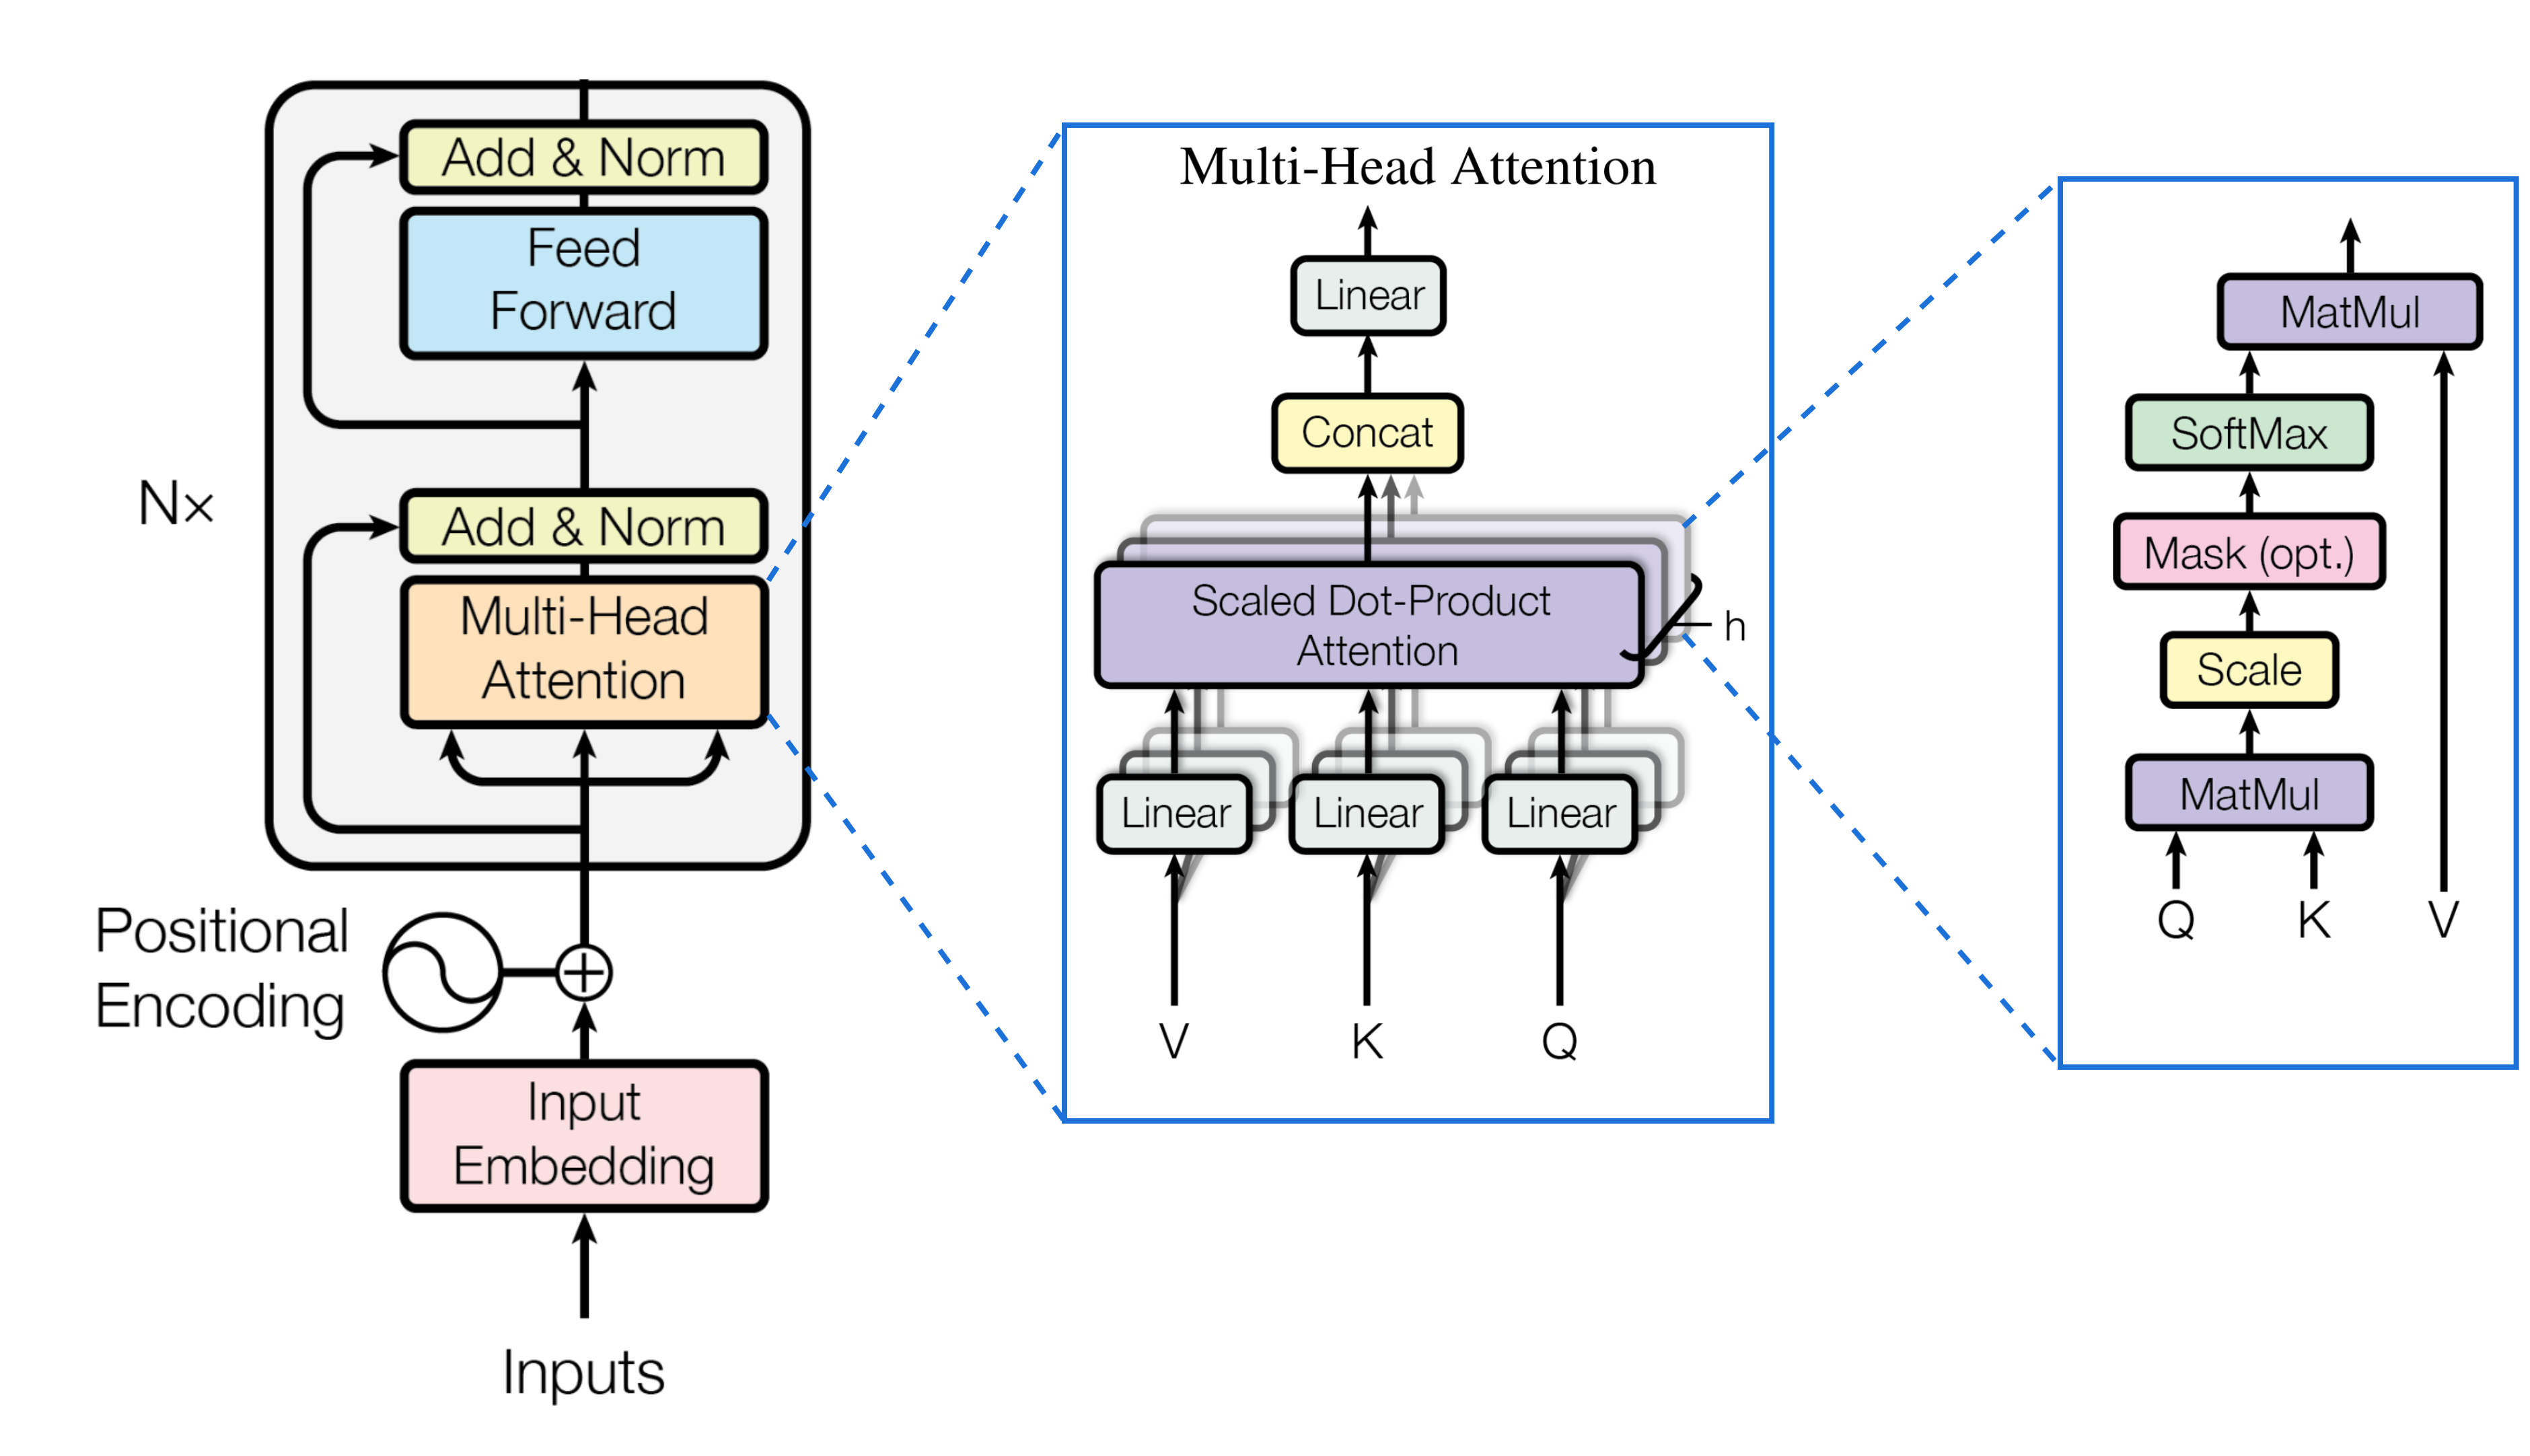
\includegraphics[width=0.95\linewidth]{figures/04_transformer/Transformer_overview.png}
    \caption{Overview of the Transformer encoder. In the first step, the inputs are embedded and positional encodings are added. Each of the $N_x$ encoder blocks contains a multi-head attention mechanism and a feedforward network. Both components are followed by layer normalization and are wrapped in residual connections, indicated by the arrows pointing to the Add \& Norm blocks. The middle panel shows the multi-head attention mechanism in more detail. Queries, keys, and values are computed by linearly transforming the inputs with their respective weight matrices. Scaled dot-product attention is then applied to these projections, and the outputs from all attention heads are concatenated and linearly transformed. The right panel illustrates the computational steps of scaled dot-product attention. This figure is adapted from~\cite{vaswani_attention_2023}.}
\label{fig:transformer_encoder}
\end{figure}

Figure~\ref{fig:transformer_encoder} illustrates an encoder-only Transformer model. The input sequence is first divided into tokens, where a token can represent a word fragment, a segment of a protein sequence, or a portion of a waveform. Each token is mapped to an embedding vector. Before entering the encoder blocks, positional encoding is added to these embeddings. 

The encoder consists of a series of identical encoder blocks, each composed of a multi-head attention mechanism followed by a feedforward network. The feedforward component closely resembles the multilayer perceptron described in section~\ref{sec:03_mlp}. 
Both components are wrapped in residual connections and followed by layer normalization, which together is denoted as Add \& Norm. Decoder blocks use similar structures but are more complex and not discussed here~\cite{murphy_probabilistic_2022, prince_understanding_2023, vaswani_attention_2023}.


\subsubsection{Input representation}
\label{sec:03_input_representation}

The input sequence is split into $n_t$ sub-sequences called tokens. In natural language processing applications, each token is then typically mapped to a learned embedding vector $\mathbf{x} \in \mathbb{R}^{d_{\mathrm{emb}}}$ representing semantic or contextual features in a continuous vector space. All token embeddings are stored in a matrix $\mathbf{T} \in \mathbb{R}^{d_{\mathrm{emb}} \times n_t}$, where each column corresponds to a token embedding~\cite{zhang_dive_2023, prince_understanding_2023}.
In contrast, our approach operates on fixed-length time-series data. Each waveform is divided into equally sized segments of 10 consecutive ADC samples, resulting in 140 uniformly spaced tokens per waveform. Each token is then projected into a 128-dimensional embedding vector via a learnable linear transformation. Using lower-dimensional embeddings can reduce training complexity but may result in underfitting. Conversely, higher-dimensional embeddings increase computational cost and risk of overfitting. 

Because attention mechanisms are inherently permutation-invariant, they lack information about the order of input tokens. Positional encoding addresses this by injecting sequence order into the model. 

The  positional encoding is implemented as a matrix $\mathbf{PE} \in \mathbb{R}^{n_t \times d_{\mathrm{emb}}}$, where $n_t$ is the number of tokens and $d_{\mathrm{emb}}$ the embedding dimension. Each row corresponds to a token and each column to a position in the embedding space~\cite{zhang_dive_2023}.
Vaswani et al. proposed a sinusoid positional embedding, where the elements are computed as:

\begin{align}
\label{eq:positional_encoding_even}
	\mathrm{PE}_{ \,i, \, 2j} & = \sin \left( \frac{i}{C^{2j/d}} \right) \,,\\
\label{eq:positional_encoding_odd}
	\mathrm{PE}_{\, i, \, 2j+1} & = \cos \left( \frac{i}{C^{2j/d}} \right)	\,,
\end{align}

\noindent where $i$ is the token index, $j$ is the embedding dimension, and $C$ is a scaling constant. We use the common choice of $C = 10^4$, which is long enough to provide a wide range of frequency scales, allowing the model to capture both short- and long-range dependencies in the sequence. Since even indices are computed with sine and odd ones with cosine, $j$ runs up to $(d/2 -1)$~\cite{vaswani_attention_2023, murphy_probabilistic_2022}. The resulting positional encoding is shown in  figure~\ref{fig:positional_encoding}.


\begin{figure}[t]
    \centering
    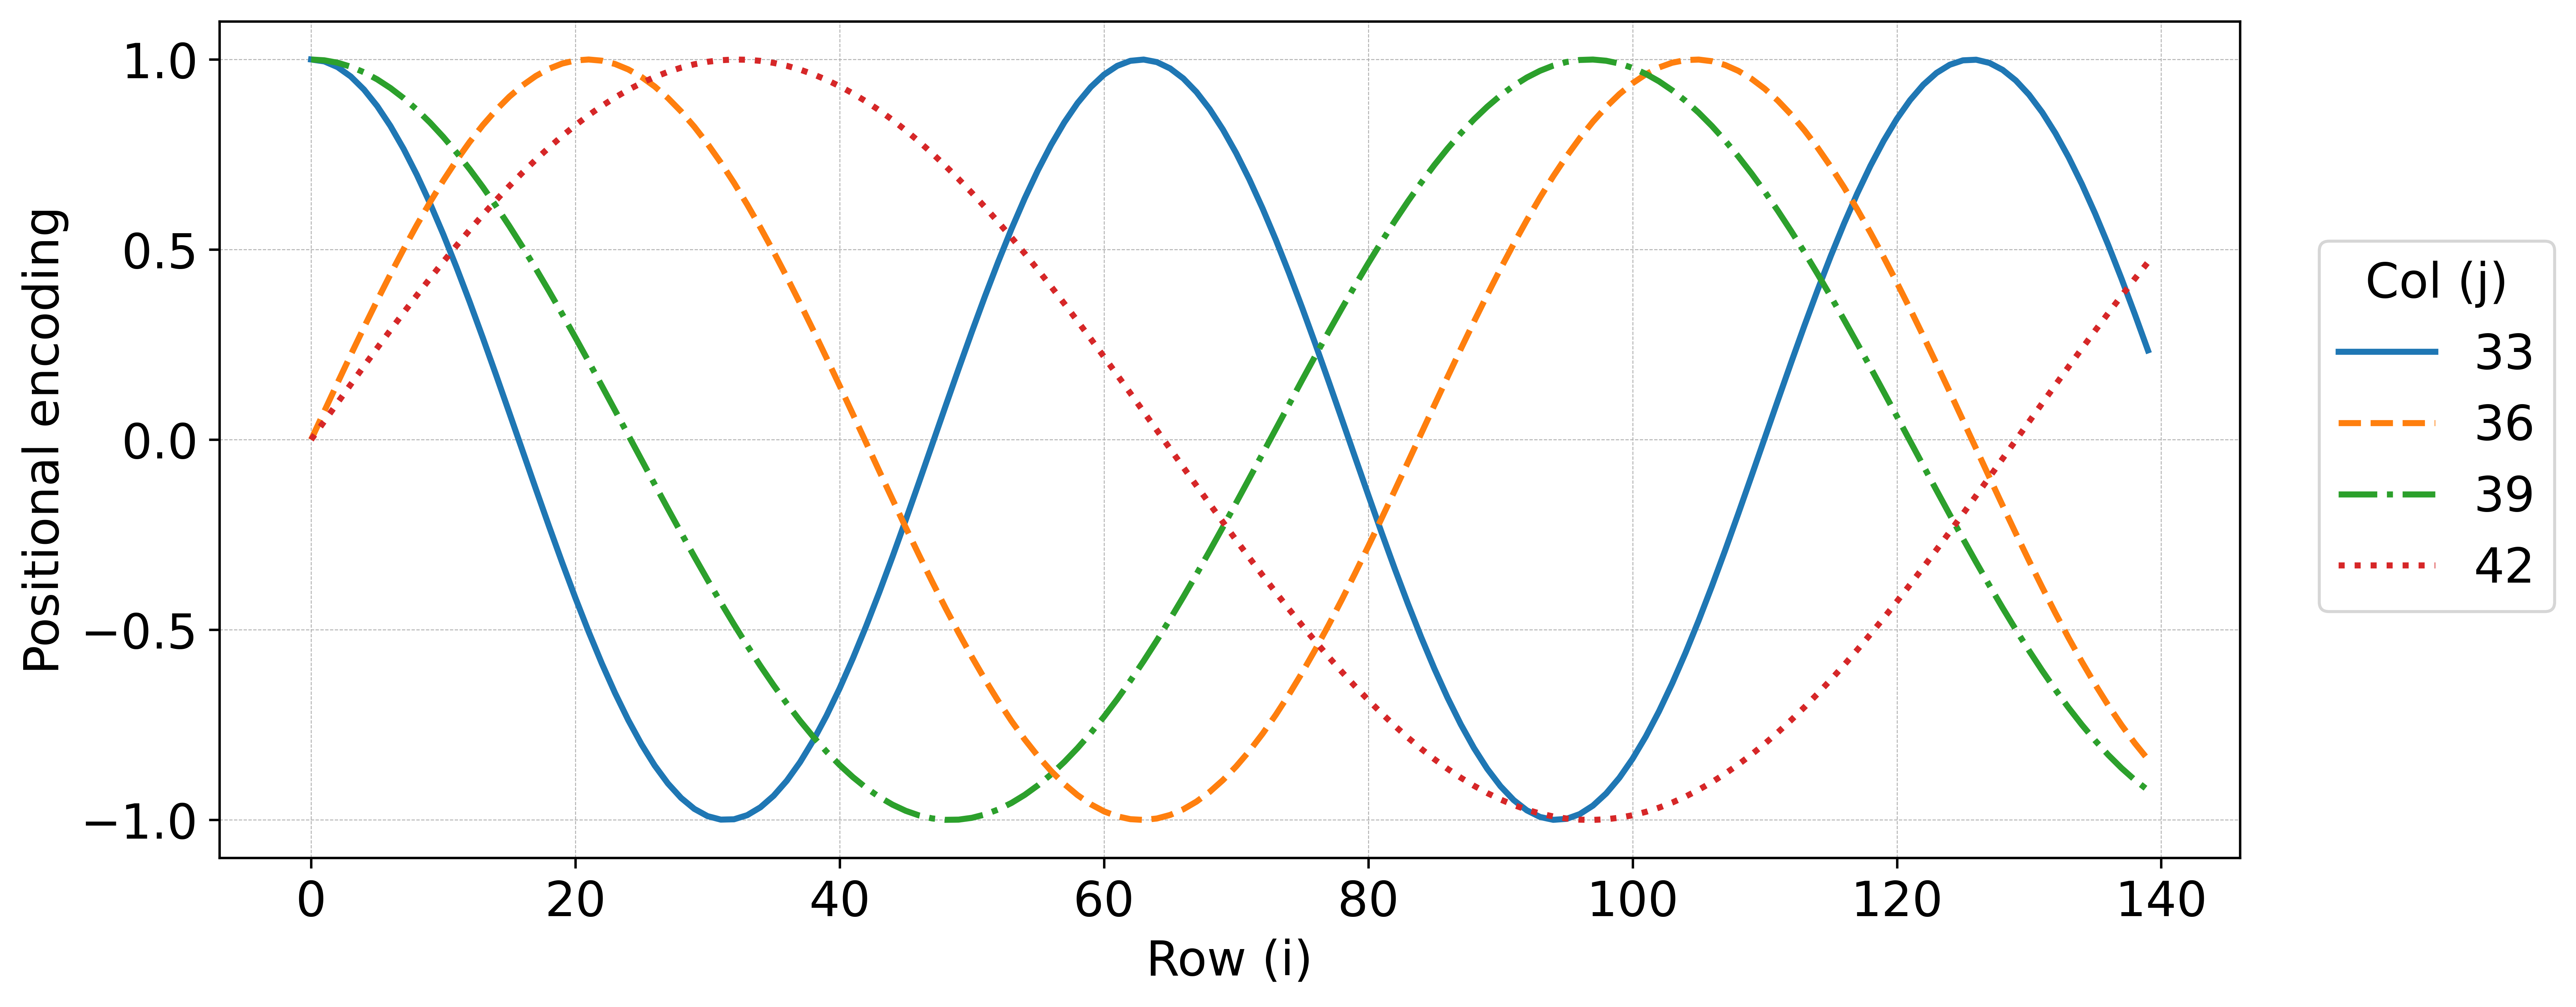
\includegraphics[width=0.95\linewidth]{figures/04_transformer/Positional_encoding.png}
    \caption{Sinusoidal positional encoding used in this work. Note that higher dimensions (columns) encode lower-frequency information. Even columns start at 0, and odd columns start at 1.} 
\label{fig:positional_encoding}
\end{figure}

Although seemingly complex, this encoding offers two major advantages. First, it allows for arbitrary sequence lengths up to $C$ without retraining. Second, the encoding for one position can be linearly computed from another. This linearity allows the model to reason about relative positions and extrapolate to unseen sequence lengths, which supports better generalization in tasks involving variable-length inputs~\cite{murphy_probabilistic_2022, vaswani_attention_2023}. For example, in a low-dimensional case with $d=2$ and $C=1$, the positional encoding $k$ steps away from position $p$ is:

\begin{align}
	\begin{pmatrix} \mathrm{PE}_{p + k, \, 0} \\ \mathrm{PE}_{p+k, \, 1} \end{pmatrix} & = 
	\begin{pmatrix} \sin \left( p + k \right) \\ \cos \left( p + k \right) \end{pmatrix} = 
	\begin{pmatrix}  \sin p \cos k + \cos p \sin k \\ \cos p \cos k - \sin p \sin k  \end{pmatrix} \\
	& = \begin{pmatrix} \cos k & \sin k \\ -\sin k & \cos k \end{pmatrix} \begin{pmatrix} \sin p \\ \cos p \end{pmatrix} \,.
\end{align}

\noindent Once computed, positional encodings are added to the embeddings $\mathbf{x}$: 

\begin{equation}
\label{eq:pos_enc_add}
    \mathbf{\tilde x} = \mathbf{x} + \mathbf{PE} \,.
\end{equation}


\subsubsection{Attention mechanism}
\label{sec:03_attention_mechanism}

The multilayer perceptron described in section~\ref{sec:03_mlp} applies a linear transformation to the input vector $\mathbf{x}$, followed by an activation function $F$. Each layer has its own set of learnable parameters.

The attention mechanism takes a different approach. Conceptually, it operates like a database: Given a set of $N$ keys $\mathbf{k}_i$ and values $\mathbf{v}_i$, a query vector $\mathbf{q}$ is used to retrieve information. 
This design allows the model to process variable-length input sequences and dynamically adapt the output based on contextual relevance. When every token attends to every other token, this mechanism allows each token to incorporate information from all other tokens, regardless of distance. This property makes attention particularly powerful for capturing long-range dependencies in sequential data. 
The general form of attention is:

\begin{equation}
\label{eq:attention}
	\mathrm{Attn}[\mathbf{q}] = \sum_{i=1}^{N} \alpha \left[ \mathbf{q}, \mathbf{k}_i \right] \, \mathbf{v}_i
\end{equation}

Here, attention is a weighted sum over the values, where each scalar weight $\alpha \left[ \mathbf{q}, \mathbf{k}_i \right]$ reflects how much attention is paid to value $\mathbf{v}_i$ given the query. These weights are computed by an attention-scoring function. In transformers, the most common method is the scaled dot product: 

\begin{equation}
\label{eq:attn_scaled_dotproduct}
	\alpha[\mathbf{q}, \mathbf{k}_i] =  \mathrm{softmax} \left( \frac{\mathbf{q}^{\intercal} \cdot \mathbf{k}_i}{\sqrt{d_k} } \right) = \frac{\exp[\mathbf{q}^{\intercal} \cdot \mathbf{k}_i / \sqrt{d_k}]}{\sum_{j=1} \exp[\mathbf{q}^{\intercal} \cdot \mathbf{k}_{j} / \sqrt{d_k}]}
\end{equation}

Scaling by $\frac{1}{\sqrt{d_k}}$ improves numerical stability. The softmax ensures all attention weights are positive and sum to one, so they act like a probability distribution over the values~\cite{prince_understanding_2023, zhang_dive_2023}. The scaled-dot product is illustrated in figure~\ref{fig:Scaled_dot_product}. 


\begin{figure}[t]
    \centering
    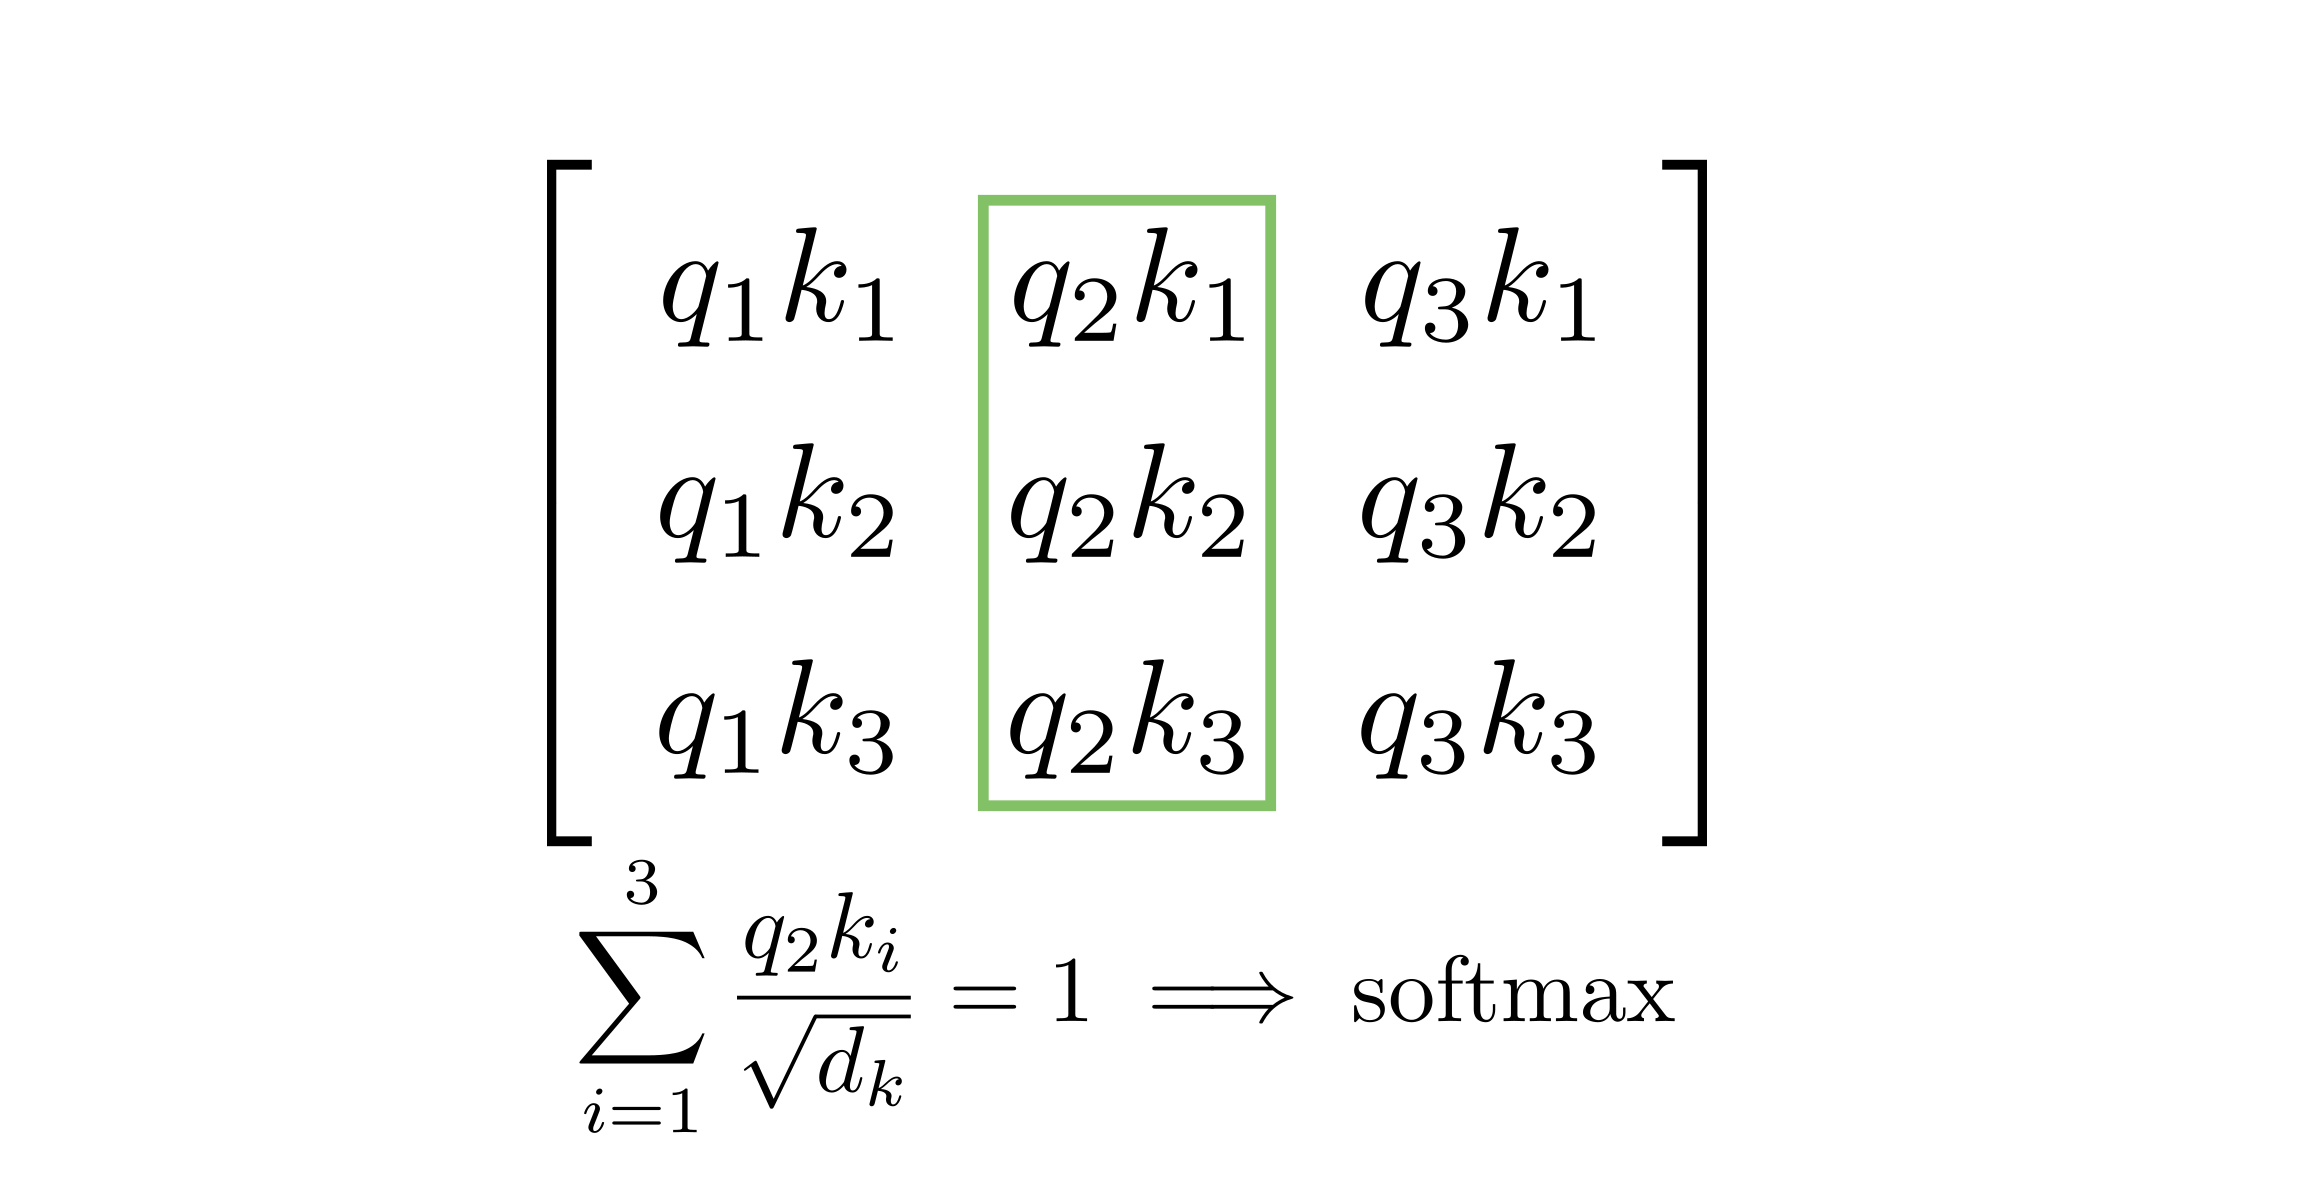
\includegraphics[width=0.75\linewidth]{figures/04_transformer/Attentionpattern.png}
    \caption{Visualization of scaled dot-product attention. Each row corresponds to a query vector $\mathbf{q}_i^{\intercal}$ and each column to a key vector $\mathbf{k}_j$. The boxed row shows attention weights from query $\mathbf{q}_2$ to all keys. These are normalized via softmax and used to compute a weighted sum over value vectors $\mathbf{v}_j$. Figure created with~\cite{the_manim_community_developers_manim_2025}.}
    \label{fig:Scaled_dot_product}
\end{figure}

In Transformer models, keys, queries, and values are computed as linear projections of the same input embeddings $\mathbf{x}_n$ using learned weight matrices:

\begin{align}
\label{eq:attn_keys}
	\mathbf{k}_n & = \mathbf{W_K} \, \mathbf{x}_n \qquad \mathbf{W_K} \in \mathbb{R}^{d_k \times d_{\mathrm{emb}}} \\
\label{eq:attn_values}
	\mathbf{v}_n & = \mathbf{W_V} \, \mathbf{x}_n \qquad \mathbf{W_V} \in \mathbb{R}^{d_{\mathrm{emb}} \times d_{\mathrm{emb}}} \\
\label{eq:attn_queries}
	\mathbf{q}_n & = \mathbf{W_Q} \, \mathbf{x}_n \qquad \mathbf{W_Q} \in \mathbb{R}^{d_q \times d_{\mathrm{emb}}} 
\end{align}

Because all three vectors are derived from the same embedding, this is referred to as self-attention:


\begin{equation}
\label{eq:self_attention}
	\mathrm{SelfAttn}[\mathbf{x}_n] = \sum_{m=1}^N \alpha \left[ \mathbf{x}_m, \mathbf{x}_n \right] \, \mathbf{v}_m \,.
\end{equation}

In practice, we vectorize the computation by stacking all embeddings into a matrix $\mathbf{X} \in \mathbb{R}^{d_{\mathrm{emb}} \times N}$, with each column $\mathbf{x}_n$ representing a token~\cite{zhang_dive_2023, prince_understanding_2023}. The keys, queries, and values are then computed in matrix form: 

\begin{align}
\label{eq:attn_queries_matrix}
	\mathbf{Q} & = \mathbf{W_Q} \, \mathbf{X} \qquad \mathbf{Q} \in \mathbb{R}^{d_k \times N} \\
\label{eq:attn_keys_matrix}
	\mathbf{K} & = \mathbf{W_K} \, \mathbf{X} \qquad \mathbf{K} \in \mathbb{R}^{d_k \times N} 
\end{align}

The self-attention can then be calculated compactly as:

\begin{align}
\label{eq:self_attn_matrix}
	\mathrm{SelfAttn}[\mathbf{Q}, \mathbf{K}, \mathbf{V}] =  \mathrm{softmax} \left( \frac{\mathbf{Q} \cdot \mathbf{K}^{\intercal}}{\sqrt{d_k} } \right) \mathbf{V} \,.
\end{align}

Instead of using a single attention mechanism, Transformers apply multi-head attention, where $h$ attention heads run in parallel. Each head computes its own self-attention using separate learned projections. The outputs of all heads are concatenated and linearly transformed:

\begin{equation}
\label{eq:multi_head_attn}
	\mathrm{MultiHeadSelfAttn}[\mathbf{X}] = \mathbf{W_C} \begin{pmatrix} \mathrm{SelfAttn}^{1}[\mathbf{X}] \\
	\vdots \\
	\mathrm{SelfAttn}^{h}[\mathbf{X}] \end{pmatrix} \qquad \mathbf{W_C} \in \mathbb{R}^{d_k \times d_k}
\end{equation}

The final projection matrix $\mathbf{W_C}$ ensures that the concatenated output has the same shape as the original input $\mathbf{X}$. A typical and efficient choice is to set $d_k = d_{\mathrm{emb}}/h$ so that the total output dimension matches the embedding dimension~\cite{zhang_dive_2023, prince_understanding_2023, murphy_probabilistic_2022}. 


\subsubsection{Transformer architecture for LEGEND waveforms}\label{sec:04_transformer_used}

Let us now consider the specific Transformer model used in this work. It was implemented by Marta Babicz in Python using the Pytorch framework~\cite{ansel_pytorch_2024}. The architecture is encoder-only and closely resembles BERT (Bidirectional Encoder Representations from Transformers), originally introduced by Google~\cite{devlin_bert_2019}.


The input data consists of physical waveforms recorded by the LEGEND-200 experiment. Each waveform spans $20.4 \;\mu$s sampled at 1400 time steps. These waveforms are segmented into $n_t = 140$ tokens, each representing 10 time steps, and embedded into a vector of size $d_{\mathrm{emb}} = 128$. After tokenization and embedding, positional encoding is added as described in section~\ref{sec:03_input_representation}. 
The model contains $n_l = 6$ encoder layers, each using 8 attention heads in parallel. Each attention block and feedforward block is wrapped in a residual connection and followed by layer normalization, following the original Transformer design. 
Altogether, the network has nearly 1.2 million trainable parameters. Roughly one-third of these lie in the attention layers, while two-thirds are trained in the feedforward network. Table~\ref{tab:model_parameters} gives a detailed parameter breakdown. 

For the task at hand -- namely analyzing long-sequence waveform data -- Transformers are particularly well suited. Convolutional neural networks and Recurrent neural networks are generally limited in capturing long-range dependencies due to their fixed receptive fields or sequential processing. By contrast, multi-head attention can focus on multiple regions of the waveform simultaneously, enabling the model to learn subtle temporal patterns beyond classical features such as A/E. The Transformer's ability to model global context, apply dynamic attention, and process sequences in parallel is particularly valuable for pulse-shape analysis. The waveforms encode rich spatial and temporal information about energy depositions in the detector, with features that range across the full waveform. 
In the following chapter, we describe how this Transformer model was trained and evaluated on waveform data, including dataset preparation, model configuration, and training procedures. 


\begin{table}[t]
\centering
\caption{Overview of the trainable parameters of the Transformer model used in this work.  The dimension of the embedding is $d_{\mathrm{emb}} = 128$, which is equal to the dimension of the keys and queries. The number of encoder layers is $n_{l} = 6$, the number of labels $n_{\mathrm{labels}} = 4$, and the number of neurons in the feedforward network $n_n = 512$. The factor 2 in the embedding comes from the fact that we embed not only the waveform but also the gradients.} 
\label{tab:model_parameters}
\begin{tabular}{|c | c | c | c|}
	\hline
	\textbf{Architecture} & \textbf{Weights} & \textbf{Bias} & \textbf{Parameters} \\
 	\hline
 	Tokenization & $d_{\mathrm {emb}}$  & - &  128 \\
 	\hline
 	Embedding & $2 \times 10 \times d_{\mathrm{emb}}$ & $2 \times d_{\mathrm{emb}}$ & 2816 \\
 	\hline
 	Keys  & $d_{\mathrm{emb}} \times d_{\mathrm{emb}} \times n_{l}$ & $d_{\mathrm{emb}} \times n_{l}$ &  99072 \\
 	\hline
   	Queries & $d_{\mathrm{emb}} \times d_{\mathrm{emb}} \times n_{l}$ & $d_{\mathrm{emb}} \times n_{l} $ & 99072 \\
 	\hline
 	Values & $d_{\mathrm{emb}} \times d_{\mathrm{emb}} \times n_{l}$ & $d_{\mathrm{emb}} \times n_{l}$ & 99072 \\
 	\hline
 	Output matrix & $d_{\mathrm{emb}} \times d_{\mathrm{emb}} \times n_{l}$ & $d_{\mathrm{emb}} \times n_{l}$ & 99072 \\
 	\hline
 	Linear layer 1 & $d_{\mathrm{emb}} \times n_{n} \times n_{l}$ & $n_{n} \times n_{l}$ & 396288 \\ 
 	\hline
	Linear layer 2 & $n_{n} \times d_{\mathrm{emb}} \times n_{l}$ & $d_{\mathrm{emb}} \times n_{l}$ & 393984 \\
	\hline
	Normalization 1 & $d_{\mathrm{emb}} \times n_{l}$ & $d_{\mathrm{emb}} \times n_{l}$ & 1536 \\
	\hline
	Normalization 2 & $d_{\mathrm{emb}} \times n_{l}$ & $d_{\mathrm{emb}} \times n_{l}$ & 1536 \\
	\hline
	Decoder & $n_{\mathrm{labels}} \times d_{\mathrm{emb}}$ & $n_{\mathrm{labels}}$ & 516 \\
	\hline
	De-embedding & $2 \times d_{\mathrm{emb}}$ & - & 256 \\
	\hline
	Total: & & & 1193348 \\
	\hline
\end{tabular}
\end{table}


